\documentclass[12pt, a4paper, twoside, openright, slovak]{book}

\usepackage[slovak]{babel}
\usepackage[utf8]{inputenc}
\usepackage[T1]{fontenc}
\usepackage{geometry}
\usepackage{epigraph}
\usepackage{subcaption}
\usepackage{hyperref}
\usepackage{enumitem}
\usepackage{tabularx}
\usepackage{afterpage}
\usepackage{multirow}
\usepackage{amsfonts}
\usepackage{amssymb}
\usepackage{listings}
\usepackage{titlesec}
\usepackage{setspace}
\usepackage{fancyhdr}
\usepackage{fancyvrb}
\usepackage[fleqn]{amsmath}
\usepackage{pdfpages}
\usepackage{nccmath}
\usepackage{csquotes}
\usepackage{diagbox}
\usepackage{ifthen}
\usepackage{algorithm}
\usepackage{algpseudocode}
\usepackage{textcomp}

\usepackage[titles]{tocloft} % TOC header same as chapter title
%\usepackage{showframe}
\usepackage{titlesec}
\titlespacing*{\chapter}{0pt}{0pt}{40pt}

\usepackage{nomencl}
\usepackage{makeidx}
\usepackage{expl3}
\usepackage{etoolbox}
\preto\tabular{\shorthandoff{-}}

\usepackage[style=iso-authoryear, backend=biber]{biblatex}
\addbibresource{literature.bib}

% Zoznam skratiek
\makenomenclature
\renewcommand{\nomname}{Zoznam skratiek a pojmov}

\makeatletter
\newcommand*{\rom}[1]{\expandafter\@slowromancap\romannumeral #1@}
\makeatother

% Empty even pages at the end of chapter
\makeatletter
\renewcommand*{\cleardoublepage}{\clearpage\if@twoside \ifodd\c@page\else
\hbox{}
\thispagestyle{empty}
\newpage
\if@twocolumn\hbox{}\newpage\fi\fi\fi}
\makeatother


% Číslo kapitoly na rovnakom riadku ako názov
\titleformat{\chapter}{\normalfont\huge\bf}{\thechapter}{1em}{}

\raggedbottom
\newcommand{\emptypage}{\newpage\thispagestyle{empty}\mbox{}\newpage}
\newcommand{\signaturespace}[2]{
  \begingroup
  \renewcommand{\arraystretch}{0}
  \begin{tabular}[t]{cc}
  \hspace*{0pt}
  \cleaders\hbox{\kern.6pt.\kern.6pt}\hskip#1\relax
  \hspace*{0pt}
  \\[0.5cm]
  #2
  \end{tabular}
  \endgroup
}

\pagestyle{fancy}
\fancyhf{}  % clear all header and footers
\fancyhead[LE]{\leftmark}
\fancyhead[RO]{\rightmark}
\fancyfoot[C]{\thepage}

\fancypagestyle{plain}{
  \fancyhf{}
  \renewcommand{\headrulewidth}{0pt}
  \fancyfoot[C]{\thepage}
}

\setlength{\headheight}{16pt}


\setstretch{1.5}
\newcommand{\SignPlace}[0] {V Bratislave, }
\newcommand{\SignDate}[0] {2023}

\usepackage{inconsolata}
\lstnewenvironment{code}{\lstset{
    basicstyle=\ttfamily\small,
    backgroundcolor=\color{gray!10},
    frame=single,
    tabsize=2,
    rulecolor=\color{black!30},
    title=\lstname,
    escapeinside={\%*}{*)},
    breaklines=true,
    breakatwhitespace=true,
    framextopmargin=2pt,
    framexbottommargin=2pt,
    inputencoding = utf8,  % Input encoding
    extendedchars = true,  % Extended ASCII
    literate      =        % Support additional characters
      {á}{{\'a}}1  {é}{{\'e}}1  {í}{{\'i}}1 {ó}{{\'o}}1  {ú}{{\'u}}1
      {Á}{{\'A}}1  {É}{{\'E}}1  {Í}{{\'I}}1 {Ó}{{\'O}}1  {Ú}{{\'U}}1
      {à}{{\`a}}1  {è}{{\`e}}1  {ì}{{\`i}}1 {ò}{{\`o}}1  {ù}{{\`u}}1
      {À}{{\`A}}1  {È}{{\`E}}1  {Ì}{{\`I}}1 {Ò}{{\`O}}1  {Ù}{{\`U}}1
      {ä}{{\"a}}1  {ë}{{\"e}}1  {ï}{{\"i}}1 {ö}{{\"o}}1  {ü}{{\"u}}1
      {Ä}{{\"A}}1  {Ë}{{\"E}}1  {Ï}{{\"I}}1 {Ö}{{\"O}}1  {Ü}{{\"U}}1
      {â}{{\^a}}1  {ê}{{\^e}}1  {î}{{\^i}}1 {ô}{{\^o}}1  {û}{{\^u}}1
      {Â}{{\^A}}1  {Ê}{{\^E}}1  {Î}{{\^I}}1 {Ô}{{\^O}}1  {Û}{{\^U}}1
      {œ}{{\oe}}1  {Œ}{{\OE}}1  {æ}{{\ae}}1 {Æ}{{\AE}}1  {ß}{{\ss}}1
      {ẞ}{{\SS}}1  {ç}{{\c{c}}}1 {Ç}{{\c{C}}}1 {ø}{{\o}}1  {Ø}{{\O}}1
      {å}{{\aa}}1  {Å}{{\AA}}1  {ã}{{\~a}}1  {õ}{{\~o}}1 {Ã}{{\~A}}1
      {Õ}{{\~O}}1  {ñ}{{\~n}}1  {Ñ}{{\~N}}1  {¿}{{?`}}1  {¡}{{!`}}1
      {°}{{\textdegree}}1 {º}{{\textordmasculine}}1 {ª}{{\textordfeminine}}1
      {£}{{\pounds}}1  {©}{{\copyright}}1  {®}{{\textregistered}}1
      {«}{{\guillemotleft}}1  {»}{{\guillemotright}}1  {Ð}{{\DH}}1  {ð}{{\dh}}1
      {Ý}{{\'Y}}1    {ý}{{\'y}}1    {Þ}{{\TH}}1    {þ}{{\th}}1    {Ă}{{\u{A}}}1
      {ă}{{\u{a}}}1  {Ą}{{\k{A}}}1  {ą}{{\k{a}}}1  {Ć}{{\'C}}1    {ć}{{\'c}}1
      {Č}{{\v{C}}}1  {č}{{\v{c}}}1  {Ď}{{\v{D}}}1  {ď}{{\v{d}}}1  {Đ}{{\DJ}}1
      {đ}{{\dj}}1    {Ė}{{\.{E}}}1  {ė}{{\.{e}}}1  {Ę}{{\k{E}}}1  {ę}{{\k{e}}}1
      {Ě}{{\v{E}}}1  {ě}{{\v{e}}}1  {Ğ}{{\u{G}}}1  {ğ}{{\u{g}}}1  {Ĩ}{{\~I}}1
      {ĩ}{{\~\i}}1   {Į}{{\k{I}}}1  {į}{{\k{i}}}1  {İ}{{\.{I}}}1  {ı}{{\i}}1
      {Ĺ}{{\'L}}1    {ĺ}{{\'l}}1    {Ľ}{{\v{L}}}1  {ľ}{{\v{l}}}1  {Ł}{{\L{}}}1
      {ł}{{\l{}}}1   {Ń}{{\'N}}1    {ń}{{\'n}}1    {Ň}{{\v{N}}}1  {ň}{{\v{n}}}1
      {Ő}{{\H{O}}}1  {ő}{{\H{o}}}1  {Ŕ}{{\'{R}}}1  {ŕ}{{\'{r}}}1  {Ř}{{\v{R}}}1
      {ř}{{\v{r}}}1  {Ś}{{\'S}}1    {ś}{{\'s}}1    {Ş}{{\c{S}}}1  {ş}{{\c{s}}}1
      {Š}{{\v{S}}}1  {š}{{\v{s}}}1  {Ť}{{\v{T}}}1  {ť}{{\v{t}}}1  {Ũ}{{\~U}}1
      {ũ}{{\~u}}1    {Ū}{{\={U}}}1  {ū}{{\={u}}}1  {Ů}{{\r{U}}}1  {ů}{{\r{u}}}1
      {Ű}{{\H{U}}}1  {ű}{{\H{u}}}1  {Ų}{{\k{U}}}1  {ų}{{\k{u}}}1  {Ź}{{\'Z}}1
      {ź}{{\'z}}1    {Ż}{{\.Z}}1    {ż}{{\.z}}1    {Ž}{{\v{Z}}}1  {ž}{{\v{z}}}1
}}{}
  

\begin{document}

\newgeometry{top=3cm, bottom=3cm, right=2.2cm, left=2.2cm}
% Obal -----------------------------------------------------------------------
\thispagestyle{empty}
{\centering
	{\Large \MakeUppercase{Slovenská technická univerzita v Bratislave}}
	\vfill
	{{\Large \MakeUppercase{Návrh učebného textu v predmete Informatika}} \par
	\vspace{2\bigskipamount}
	{\Large \MakeUppercase{Záverečná práca \\ Doplňujúceho pedagogického štúdia}}}
	\vfill
}
{\large  
\begin{flushleft}
{\Large 2023 \hfill
Bc. Miroslav Hájek}
\end{flushleft}
}
\emptypage


% Titulný list
\pagenumbering{roman}
\thispagestyle{empty}
{\centering
	{\Large \MakeUppercase{Slovenská technická univerzita v Bratislave}} \par
	\vspace{\bigskipamount}
	{\Large  \MakeUppercase{Ústav Manažmentu}}
	\vfill
	{{\Large \MakeUppercase{Návrh učebného textu v predmete Informatika}} \par
	\vspace{2\bigskipamount}
	{\Large \MakeUppercase{Záverečná práca \\ Doplňujúceho pedagogického štúdia}}}
	\vfill
}
{\large 
\begin{flushleft}
\begin{align*}
& \text{Vedúci záverečnej práce:} && \text{doc. Ing. Gabriela Pavlendová, PhD.} \\
& \text{Bratislava, 2023} && \text{Bc. Miroslav Hájek}
\end{align*}
\end{flushleft}
}%

\emptypage

\newgeometry{top=2.5cm, bottom=2.5cm, right=2cm, left=3.5cm}
 % Čestné prehlásenie
\thispagestyle{empty}
\vspace*{\fill}
\section*{Čestné prehlásenie}
Čestne vyhlasujem, že som túto prácu vypracoval samostatne, na základe konzultácií
a s použitím uvedenej literatúry.

\vspace{3\medskipamount}\noindent
\SignPlace \SignDate \hspace*{\fill} \signaturespace{5cm}{Bc. Miroslav Hájek} 

\emptypage
\thispagestyle{empty}
\section*{Abstrakt}
Záverečná práca sa venuje tvorbe učebníc so zameraním na organizáciu a na obsahovú štruktúru systému úloh podľa náročnosti, tak aby boli všestranne podporné didaktické funkcie učebného textu. Za týmto účelom sa predstavuje inovatívna zbierka úloh z programovania so vzorovými riešeniami v jazyku Python pre stredné školy vo všeobecno-vzdelávacom vyučovacom predmete informatika. Problémové cvičenia sú po vzore súťažných úloh zasadené do kontextu krátkych príbehov, ktoré motivujú žiaka k užitočnosti konkrétnych algoritmov a programov. Aplikačné oblasti sú volené s prihliadaním na rozvoj medzipredmetových vzťahov. Široká dostupnosť zbierky je podporená prezentáciou v hypertextovom priestore webu. Kolaboratívna rozšíriteľnosť sa umožňuje vypracovaním metódy stanovujúcej pevnú predlohu úlohy, požiadaviek na kvantitatívne vlastnosti jej znenia a zaradenie do zbierky podľa témy, funkcie a poznávacej úrovne. Výsledkom je sada problémových úloh v súlade so štátnym vzdelávacím programom a cieľovými požiadavkami na maturitnú skúšku, ktorá má aktivizovať žiakov v problémovom vyučovaní a dopomáha k samostatnej domácej príprave. \\

\textbf{Kľúčové slová:} problémové vyučovanie, učebnice, zbierka úloh, informatika, základy programovania

\emptypage

\thispagestyle{empty}
\section*{Abstract}
The final thesis is aimed at the textbook design with a focus on the organization and content structure of the system of problems according to difficulty so that the didactic functions of the teaching text are supported comprehensively. For this purpose, a collection of programming problems with sample solutions in the Python language is presented for secondary schools in the general education subject of computer science. Following the model of competition problems, problem exercises are set in the context of short stories, which motivate the student to the usefulness of specific algorithms and programs. Application areas are chosen to develop interdisciplinary relationships. The wide accessibility of the textbook is supported by presenting them in the hypertext environment of the web. Collaborative extensibility is made possible by developing a method establishing a fixed template of the problem, requirements for the quantitative properties of its wording, and inclusion in the textbook according to topic, function, and cognitive level.
The result is a set of problems in the scope given by the state educational program and the target requirements for the matura exam, which is supposed to activate students in problem-based teaching and help with individual home preparation. \\

\textbf{Keywords:} problem-based learning, textbooks, collection of problems, Computer science, Programming basics
\emptypage 

% Obsah
\renewcommand{\contentsname}{Obsah}
\pagestyle{empty}
\tableofcontents{}
\emptypage

\pagestyle{fancy}
% Kapitoly
\pagenumbering{arabic}

\chapter{Úvod}
Rýchly vývoj informatiky ako vedy za posledné desaťročia, rapídny technologický rozvoj vedúci k zvýšeniu dostupnosti prostriedkov výpočtovej techniky a nástup inovatívnych prístupov vo výučbe umocňuje nedostatok moderných kvalitných vzdelávacích materiálov pre stredné školy. Na vzdelávanie informatiky na úrovni vyššieho sekundárneho vzdelania nevplýva ani tak posun v podstatných princípoch odboru, ale skôr výskyt nových informačných a komunikačných technológií prinášajúcich predtým nepoznané výzvy do spoločnosti. Nemenej podstatný dopad majú schopnosti nástrojov, čiže vlastností softvérového vybavenia a jeho používateľského rozhrania

Pre niektoré oblasti, ako sú kybernetická bezpečnosť alebo programovanie vychádzajú v súčasnosti už aktuálne učebnice, ale častokrát sú školám nedostupné najmä z ekonomických dôvodov. Poznatky v tlačených učebniciach zároveň zvyknú rýchlo zastarávať, preto sa preferujú elektronické knihy. E-knihy majú zasa z pohľadu vyučovacieho procesu úskalia ohľadom ich prístupnosti a prevládajúceho tradicionalizmu.

Význačné zmeny sa udiali v programovacích jazykoch ako nástrojoch na formálny zápis algoritmov. Ovplyvnili výber prostredí na programovanie a jazykov pre použitie vo vzdelávaní a postupnosť v osvojovaní prvkov jazyka. Nové verzie neustále prinášajú úpravy syntaxe a údajových štruktúr.

V záujme udržania kroku s najnovšími relevantnými poznatkami v odbore a stavom technológií, sú učitelia často nútení pripravovať si vlastné učebné texty. Napomáhajú im k tomu internetové zdroje a e-learningové knižnice. Ponechávajú však časovo náročný výber adekvátnych článkov a vyváženú skladbu cvičení na kreativite učiteľa. Na prvý pohľad sa to môže javiť prospešné pre individualizáciu výučby. Realizácia nebýva nikdy ideálna, tak aby žiakom poskytla rozmanité úlohy na samostatnú domácu prípravu.

Na vyučovacích hodinách by mala dobrá učebnica vhodne podnecovať a podporovať problémové vyučovanie, ktoré aktivizuje žiakov k hlbšiemu ovládaniu preberanej témy. Okrem iných časových a priestorových obmedzení vplývajúcich na výber učebnej metódy, vedie učiteľa nedostupnosť usporiadaného učebného textu na sprevádzanie učivom, hlavne k využitiu frontálneho výkladu.

V svojpomocnej tvorbe učebníc všeobecnovzdelávacieho učebného predmetu informatika sa zameriavame na vzdelávací štandard algoritmické riešenie problémov podľa štátneho vzdelávacieho programu. V snahe preniesť úsilie v triede pri osvojovaní učiva vo väčšej miere na žiaka, vychádzame z potreby zostavenia zbierky úloh z programovania pre stredné školy k použitiu v škole aj na doma. Nevyhnutné zložky hodné komplexného posúdenia sú obsahová a formálna rovina.

Na obsah zbierky kladieme nároky na vyvážené pokrytie dôležitých typov úloh na viacerých kognitívnych úrovniach v súlade s princípmi formulácie úlohy aj systematickým usporiadaním úloh. Spôsob začlenenia riešení do zbierky a ich fáza konfrontovania s postupmi žiakov je tiež neoddeliteľnou súčasťou učebného textu ako celku. Na predchádzanie straty aktuálnosti textov budeme požadovať čo najväčšiu nezávislosť úloh na programovacom prostredí a jazyku.

Po formálnej stránke máme záujem navrhnúť ,,živú učebnicu'', kde by mohli učitelia v online prostredí postupne dopĺňať nové úlohy do jednotlivých častí zbierky. Na tento účel prispôsobujeme existujúcu metodiky hodnotenia náročnosti textu a zaraďovania úloh do systému úloh podľa príslušných kritérií. Prihliada sa pritom na obsahové zameranie v rámci tematických okruhov podľa znenia zadania. Namiesto opakujúcich sa typov cvičení sa nájde náhrada vhodným preformulovaním.

V hlavnej časti práce preskúmame teóriu tvorby učebníc s ohľadom na funkcie, skvalitňovanie učebného textu a na nástrahy pri presune do elektronickej podoby. Ďalej sa venujeme zostrojeniu adekvátneho a rozšíriteľného systému úloh podľa zbierok príkladov z matematiky. Nasleduje prehľad a rozbor súčasných učebníc programovania a zbierok úloh. V praktickej časti predstavíme konkrétne úlohy so vzorovými riešeniami a hodnotením zaradenia či náročnosti úloh. Nakoniec prediskutujeme typické vlastnosti textu úloh po obsahovej a grafickej stránke.

\chapter{Tvorba edukačných materiálov} 
Súčasný stav problematiky tvorby edukačných materiálov obsahuje zákonitosti stavby a funkcií učebnice, odporúčania pri písaní zrozumiteľných učebných textov a rozvrhovaní didakticky správneho systému úloh v zbierke. Tiež porovnáme doterajšie učebnice programovania pre stredné školy navzájom a vzhľadom na štátny vzdelávací štandard. 

\section{Učebnica}
Základným prameňom poznatkov a nositeľom obsahu vzdelávania je učebnica, ktorá patrí medzi čelných predstaviteľov pedagogických textov. Predstavuje jadro zoskupujúce okolo seba ostatné učebné prostriedky (\cite{zujev_ako_1986}). V medziach učebných osnov vymedzuje obsah základného učiva s doplnením o rozširujúce učivo, pričom rozsah osnovy učebnice nemusí byť totožný s učebnými osnovami (\cite{mlady_tvorba_1988}). 

Učebnica pomáha žiakom s osvojením si obsahu učiva, čím podporuje všetky súvisiace čiastkové činnosti: precvičovania, opakovania, systematizácie a integrácie. V edukačnom procese učebnica pôsobí aj výchovne, čím vplýva na formovanie postojov, motívov a záujmov. Odlišuje sa v tom od iných kníh a texov, pretože má priamu spätosť so získavaním a spracovaním faktov, pojmov a vzťahov žiakmi. Efektívne tak smeruje dosiahnutie výchovno-vzdelávacích cieľov vyučovacieho predmetu (\cite{gavora_ziak_1992}). Učebný program žiaka a vyučovací program učiteľa je ideálne v učebnici pochytený a odráža sa do scenáru učebného a vyučovacieho procesu. Hlvaná časť učebnice prestavuje súbor úloh určených na aktívne riešenie (\cite{pavlovkin_ziak_1989}).

Podľa školského zákona sa učebnica spolu s učebným textom a pracovným zošitom zaraďuje medzi edukačné publikácie. Na vzdelávanie sa používajú edukačné publikačné schválené ministerstvom školstva alebo zodpovedajúce princípom a cieľmi výchovy a vzdelávania (\cite{skolsky_zakon}). Princípy súvisiace s vlastnými vzdelávacími materiálmi sú v duchu rovnoprávnosti, rovnocennosti, zodpovednosti, tolerancie a vyváženého rozvoja osobnosti a zdokonaľovania vzdelávania podľa výsledkov výskumu a vývoja.

\subsection{Didaktické funkcie učebnice}
V učebnici pôsobí viacero naviazných a prelínajúcich sa vlastností vystupujúcich vo výchovno-vzdelávacom procese (\cite{zujev_ako_1986}), ktoré sú popísané bez stanoveného poradia dôležitosti:
\begin{itemize}
\itemsep0pt
\item \textbf{Informačná funkcia}: sa sústreďuje na stanovenie povinného rozsahu informácií pri štúdiu nevyhnutných na zapamätanie.
\item \textbf{Transformačná funkcia}: spočíva v didaktickom transfere poznatkov vedného odboru na obsah učiva v zrozumiteľnej a pútavej podobe, a zaroveň sa berie do úvahy na vekové a kultúrne osobitosti žiakov. Nabáda na výber vzdelávacích metód a uľahčuje aktivizáciu žiaka pri cvičeniach a úlohách prieskumného charakteru. Pri transformácii znalostí sa hľadí sa aj na potreby profesijného života a spoločenského očakávania od absolventov.
\item \textbf{Systematizačná funkcia}: pri objasňovaní učiva zabezpečuje následnosť poznatkov, postupný nárast náročnosti a vedie k metódam vedeckej systematizácie.
\item \textbf{Usmerňujúca funkcia}: slúži k upevňovaniu vedomostí napomáha v orientácii sa v nich a zapojením ich do praktických druhov činností. Vyžaduje sprevádazanie navrhnutými aktivitami pod vedením učiteľa.
\item \textbf{Motivačná funkcia}: pobáda túžbu a schopnosti žiakov na samostatné získavanie vedomostí.
\item \textbf{Integračná funkcia}: ucelene spája poznatky žiakov nadobudnuté z ich rozličných činností.
\item \textbf{Koordinačná funkcia}: zapája ku vzťahu k študovanému predmetu informácie z masovo-komunikačných prostriedkov. 
\item \textbf{Výchovná funkcia}: súčasne tiež rozvíjajúca funkcia, ktoré spočívajú v zladenom formovaní čŕt osobnosti žiaka.
\end{itemize}
Uvedené didaktické funkcie zabezpečujú komplexné pôsobenie učebnice na rozvoj kognitívnych a afektívnych schopností žiaka. Pri ich prepojení v učebnom texte dochádza nielen k nadobudnutiu nevyhnutných vedomostí a zručností na zvládnutie vyučovacieho predmetu, ale aj rozvoj kľúčových kompetencií a medzi nimi pripravenosti k všestrannejšiemu učeniu sa.


\subsection{Prvky učebnice}
Aby učebnica plnohodnotne napĺňala svoje mnohé poslania je poskladaná z \textbf{prvkov textového i mimotextového charakteru}, ktoré podnecujú aktívne kognitívne procesy a umožňujú zapojenie zvoleného učebného štýlu čitateľa. Zaradenie súčastí učebnice do členenia jej podsystémov nie je striktné, ale riadi sa dominantnou funkciou danej časti (\cite{zujev_ako_1986}).

Text v učebnici je súhrn viacerých viet, ktoré sú prostriedkom na odovzdanie informácií žiakom podľa komunikačného zámeru autora. Z povahy súvislého písaného jazykového prejavu sa vyznačuje kohéziou a koherenciou. Kohézia je súdržnosť textu na úrovni vzájomnej nadväznosti medzi vetami za použitia gramatických, lexikálnych a grafických jazykových prostriedkov. Najčastejšie sa uplatňujú gramatická zhoda medzi nadradeným a podradeným slovným druhom alebo vetným členom, opakovanie výrazu ďalej v texte, synonymá, a interpunkčné znamienka. Koherencia je zase tématická spojitosť textu, keď sa z hlavnej rozvíjajú vedľajšie myšlienky   (\cite{gavora_ziak_1992}). 

Podľa úlohy, ktorú zohráva text v predstavovaní učebnej látky sa rozlišuje \textbf{základný, doplňujúci a vysvetľujúci text}. Základný text je určený ako povinný na osvojenie pre zvládnutie problematiky. Podľa typu činností motivovanej základným textom sú povšimnuté teoretické poznávacie texty považované tiež za výkladovú zložku zastávajúcu informačnú funkciu vysvetľovania a komentovania nového učiva. Kdežto u inštrumentálno-praktických textov, alebo aj nevýkladovej zložky prevláda transformačná funkcia premietajúca sa do otázok, úloh a cvičení. Doplňujúci text prehlbuje rozsah učebných osnov dodatočňou argumentáciu vplývajúcej na rozumovú a emočnú stránku. Regulovanie poznávacej činnosti má na starosti vysvetľujúci text, ktorý dáva základný text do súvislostí (\cite{zujev_ako_1986}).

Mimotextové zložky nachádzajúce sa v učebnici sú zatrieďované na \textbf{aparát organizácie osvojovania, ilustračný materiál, a orientačný aparát}. Na organizáciu osvojovania slúžia prehľadové tabuľky, otázky a úlohy spolu s odpoveďami, ktoré v závislosti od kontextu sú spadajú do základného textu. Ilustrácie prevažne graficky dotvárajú textovú zložku, s ktorou sú vo vzťahovej rovine buď nadradenosti ako vedúce ilustrácie, rovnocennosti, alebo podradenosti ako doplnkové ilustrácie. Súvislosť medzi textom a ilustráciou sa spozná, podľa toho či text opisuje ilustráciu, vtedy je text podradený, alebo ilustrácia slúži na dokreslenie sitúcie. Typickými príkladmi ilustrácií sú obrázky, schémy, plány, diagramy, grafiky, mapy. Orientačný aparát slúži na zdôraznenie slovných spojení alebo myšlienok cez tlačové zvýraznenia a symbolické značenie, alebo opakuje prvky z hlavnej časti v zhutnenej podobe na navigáciu v knihe, v čom spočíva úloha napríklad predhovoru, obsahu, a registrov (\cite{zujev_ako_1986}).

Tradičná redakčná výroba učebnice dbá na ustálené metódy a organizovanú spoluprácu pre kontrolu správnosti obsahu po odbornej stránke a dohliada na gramatickú, pravopisnú a štylistickú úpravu (\cite{mlady_tvorba_1988}). Zasadzuje sa o koordináciu činnosti autorských kolektívov, tak aby umožnila zosúladiť všetky dôležité prvky učebnice najmä však súhru textovej a grafickej časti. Osvedčené pracovné postupy redakcie zabezpečujúce zahrnutie podstatných zložiek učebnice začínajú vypracovaním jej osnovy, príprave materiálov a podkladov, následne príprave rukopisu a obrazových predlôh v čase vymedzenom stanoveným harmonogramom, ktoré prechádzajú korektúrou, a celkové snaženie je zavŕšené vydaním učebnice a získaním doložky ministerstvom školstva podľa osobitého predpisu. Tvorba vzdelávacích materiálov priamo učiteľmi nie je až tak rigidná, ale navádza na zmysluplnú organizáciu práce.

\subsection{Multimediálne prostredie}
Postavenie výuky informatiky okolo počítačov a súvisiaceho prídavného vybavenia vedie k prirodzenej snahe uspôsobovať edukačné materiály naskýtajúcim sa podmienkam. Tým môžu učebné texty zúžikovať príležitosti pre obohatenie ich obsahu multimédiami a hypertextovými prepojeniami. Princípy uplatňujúce sa pri tvorbe klasických učebníc sa nevyhnutne prenášajú aj na tvorbe multimediálnych učebníc, pretože rovnako zostávajú publikáciami uspôsobených ku didaktickej komunikácii (\cite{krotky_nove_2015}).

Množstvo existujúcich učebníc prechádza do online prostredia zo svojej pôvodne knižnej úpravy na zvýšenie ich atraktívnosti a pohodlia pri prístupe k nim. Ani vznik učebnice určenej primárne pre elektronické médium však ešte nezaručuje využitie ponúkaného potenciálu na skĺbenie inovatívnych vyučovacích metód a ponúknutých technických vymožeností. Preto sa odlišujú učebnice podľa náročnosti prítomných konštrukcií na \textbf{jednoduché, komplexné a pokročilé učebnice} (\cite{krotky_nove_2015}).

Jednoduché učebnice sú elektronické obrazom svojich papierových vzorov bez uplatnenia akýkoľvek nových rozširujúcich možností. Komplexné učebnice získame zakomponovaním multimediálnych prvkov, zastúpených prevažne zvukmi, obrázkami, animáciami, videom, a vložením  hypertextových odkazov smerujúcich dovnútra vlastného obsahu a na externé webové portály a ďalší multimediálny obsah. Pokročilé učebnice navyše pozostávajú s interaktívnych prvkov aktívne prispôsobujúcich tok informácii a manipulácie s nimi cez tlačidlá, posuvníky kontextové nápovedy, a príbuzné ovládanie. Nadstavbou pokročilej učebnice je edukačný softvér.

\textbf{Interaktívne personalizované úlohy} slúžiace na obohatenia osvojenia vedomostí z multimediálnej učebnice sa snažia o zníženie kognitívnej záťaže pri návrhu používateľských rozhraní, aby sa žiak mohol sústrediť výhradne na osvojované učivo skôr než na obtiaže s komplikovanými krokmi na dosiahnutie vytýčených zámerov vo virtuálnom priestore. Aplikované teórie súvisia s obmedzeniami kapacity krátkodobej pamäte. 
\textbf{Teória kognitívnej záťaže} odporúča eliminovanie vonkajšej (\emph{extraneous}) kognitívnej záťaže cez zjednodušenie kompozície zobrazovaných prvkov. Vonkajšia kognitívna záťaž zaberá miesto vnútornej (\emph{intrisic}) a konceptuálnej (\emph{germane}) záťaže, ktoré sú potrebné na riešenie samotnej úlohy (\cite{uhercik_vyznam_2012}). \textbf{Teória duálneho kódovania} hovorí, že verbálne a neverbálne podnety sú v pamäti kódované zvlášť, čím sa zvýši počet položiek v krátkodobej pamäti pokiaľ pochádzajú z odlišného zdroja (\cite{mishra_interactive_2005}). 

\textbf{Pokyny pre multimediálne úlohy} nasledujú kognitívne princípy, ktoré sa odvíjajú od schopnosti človeka vstrebávať nové podnety. Multimediálny princíp tvrdí, že ku optimálnejšiemu učeniu dochádza keď pokyny obsahujú obrázky a texty spoločne ako samostatne. Princíp modality uprednostňuje zvukovú nahrávku a animáciu pred animáciou s textom. Príníp redundancie vylučuje nadbytočné elementy, ktorým je vložený text v prípade zvuku a animácie. Princíp súdržnosti je za vynechanie nadbytočných slov, obrázkov a zvukov. Signalizačný princíp vnáša do prostredia nápovedy na usmernenie pozornosti a orientácie sa. Spojitosť v čase a priestore navádza na radšej súčasné ako postupné zobrazenie súvisiaceho textu a obrázkov. Princíp segmentácie odporúča rozčleniť na animáciu so sprievodným slovom na kratšie učiacim sa kontrolované časti (\cite{mishra_interactive_2005}). 

\subsection{Skvalitňovanie učebného textu}
Vylepšenia v učebných textoch sa uskutočňujú na základe teoretických východísk z porozumeniu textu pri \textbf{čítaní ako psycholingvistickej činnosti}. Na úspešné odhalenie komunikačného zámeru pozná recipient vzťah medzi objektívnou realitou a na ňu odkazujúce prvky textu, medzi jednotlivými prvkami textu a medzi textom a doterajšími znalosťami prijímateľa (\cite{gavora_ziak_1992}). 

Práve operáciou elaborácie sa nachádzajú asociácie v prečítanom texte s už nadobudnutým sémantickými a epizodickými znalosťami a vizuálnymi predstavami, pokiaľ existuje také spojenie. Inferencia umožňuje doplnenie zamlčaných informácii v texte, ktoré vyplývajú z opísaných pričinno-dôsledkových súvislostí (\cite{gavora_ziak_1992}).

Počas zvnútorňovania edukačného textu dochádza k postupu od jeho porozumenia bez vzťahu k iným textom, cez prevod na parafrázy a symbolický zápis, cez interpretáciu vnášajúcej odlišný pohľad na prečítané, až ku extrapolácii inovatívnych záverov a schopnosti predpovedať dôsledky (\cite{gavora_ziak_1992}). 

Na objasnenie nových konceptov je teda prospešné, ak sú úvadzané východiskové situácie povedomé a autorova predstava sa zhoduje s čitateľovou. Čítaním môže nastať neporozumenie v tzv. \textbf{mikroštruktúre textu}, to sú slová, vety, vzťahy medzi vetami, či štruktúra textu. Neznámym slovám dokážeme predchádzať ich vhodným výberom usúdenej z náročnosti pojmu. Taxonomické normy zachytávajú typickosť pojmov, tým že ho spájajú s názvom nadradenej kategórie. Zložité vety odkazujúce sa vedľajšou vetou na vzdialené slová a včlenené prívlastkové vety by mali byť radšej rozdelené na dve vety. Pozornosť treba venovať neopomenutiu podstatných spájajúcich slov. 

\textbf{Zložitosť textu} sa opisuje kvantitatívnymi charakteristikami, prejavujúce sa v čitateľnosti a náročnosti texu. \textbf{Čitateľnosť} sa zvykne merať dĺžkou viet alebo výskytom neobvyklách slov. Jednou z mnohých mier čitateľnosti je Gunning \emph{Fog index} v prijateľnom rozsahu pre stredné školy do skóre 14 (Vzorec~\ref{equ:fog-index}) (\cite{drahosova_hodnotenie_2014}). 

\textbf{Náročnosť} textu vychádza z lexikálnych a syntaktických faktorov, ktoré pokladajú na škálu zložitosť toho čo je povedané a akým spôsobom je to zapísané. \emph{Průchová modifikácia Nestlerovej metódy} zisťuje obtiažnosť na vzorkách výkladového textu učebnice zohľadnením syntaktickej a sémantickej náročnosti  v bodovom rozpätí pod 20 bodov (nízka obtiažnosť) a nad 60 bodov (vysoká obtiažnosť) (Vzorec \ref{equ:nestler-method}) (\cite{drahosova_hodnotenie_2014}). Textu vyjadrujeme tiež inferenčnú záťaž, teda nutnosť vyvodzovania vzťahov čitateľom, sa znižuje umiestnením podobných myšlienok za sebou (\cite{pavlovkin_ziak_1989}).

\begin{ceqn}\begin{align}
0.4 \cdot \left(\left(\frac{\sum slova}{\sum vety}\right) + 
\left(\frac{\sum \text{slova nad 2 slabiky}}{\sum slova}\cdot 100\right)\right)
\label{equ:fog-index}
\end{align}\end{ceqn}

\begin{equation}\begin{split}
& 0.1 \cdot \left(\frac{\sum slova}{\sum vety}\right) \cdot  \left(\frac{\sum slova}{\sum slovesa}\right) + \\
& \left(\frac{\sum pojmy}{\sum slova}\right) \cdot \left(\frac{\sum P_1 + 3\sum P_2 + 2\sum P_3 + 2\sum P_4 + \sum P_4}{\sum slova}\right)
\label{equ:nestler-method}
\end{split}\end{equation}

Ku kvalite textov učebnice prispieva aj \textbf{makroštruktúra textu}, čiže rozčlenenie tématických okruhov na kapitoly a tie na texty. Na poskytnutie nadhľadu slúžia typografické zvýraznenia hrubým písmom alebo oddeľujúcim práznym priestorom, nadpisy rôznych veľkostí na rozlíšenie tém a podtém, kľúčové vety vyjadrujúce hlavnú myšlienku, a uvádzajúce či rekapitulúce otázky pobádajúce čiateľa na aktívne prijímanie materiálu (\cite{pavlovkin_ziak_1989}). Nemenej znateľná pri čítaní je primerane jednoduchá grafická úprava neodpútavajúca pozornosť od obsahu. Prehľadnosť sa vylepšuje nastavením ľahko čitateľného písma s veľkosťou odrážajúcou hierarchiu celkov, riadkovaním do bloku, a zalamovaním príkladov v celku na jednu stranu (\cite{mlady_tvorba_1988}).

Na hodnotenie kvality učebníc sa uplatňujú experimentálne, expertné a štatistické metódy. V autentickom školskom prostredí môžeme experimentálne overovať a porovnávať navrhovanú učebnicu so staršou zaužívanou. Pozorovatelia učebnice ako sú experti, učitelia a žiaci hodnotia rozličné vlastnosti s ktorými prichádzajú do kontaktu, napríklad primeranosť, metodické spracovanie, zaujímavosť, zložitosť. Štatisticky sa kvantifikuje rozsah textu určený na vyučovaciu jednotku, čitateľnosť a náročnosť textu.

Výskum Drahošovej sumarizuje nasledujúce techniky pre pedagogickú prax na zlepšovanie zrozumiteľnosti učebného textu. Ohľadom výberu slov odporúča uprednostniť bežné slová, opísateľné pojmy a aktívne slovesá, zároveň sa vyhýbať nepotrebným slovám. V rovine štylistiky by sa malo písať s priblížením sa bežne hovorenej reči, v jednduchých celkoch a krátkych vetách. Myšlienky textu vyjadrovať adresne a presvedčivo s opieraním o skúsenosti čitateľa (\cite{drahosova_hodnotenie_2014}).

\section{Systém úloh v zbierke}
Skupina úloh sa označuje systémom úloh, keď plní konkrétnu didaktickú funkciu v súlade s učebnými cieľmi, štruktúrou poznávacieho procesu a podmienkami učebného procesu sa označuje systém úloh (\cite{mindakova_tvorba_2008}). Otázky na precvičovania učiva sa vyznačujú špecifikami oproti výkladovému textu, prevažne tým že ich vyriešenie bezpochyby vyžaduje aktívnu činnosť žiaka na rôznych úrovniach myslenia. Učiteľ v tomto štádiu pozoruje postup žiakov pri vypracovaní úloh a na základe ich vonkajších prejavov posudzuje a usmerňuje ich činnosť k želanému cieľu. Kritické je stanoviť následnosť a hierarchiu úloh, tak aby umožňovali kontinuálny rozvoj žiaka. V teminológii B.~F.~Skinnera vyvinúť program výučby.   

\subsection{Psychologické východiská}
Návrh systému úloh sa potýka s otázkami žiackej motivácie riešenia úloh, diferenciácie úloh vzhľadom na individuálne osobitosti žiakov, vhodného zoradenia úloh od jednoduchších k zložitejším a spôsobu merania stupňa zvládnutia učiva. Nie je očakávateľné, že všetky témy budú samy osebe atraktívne. Dieťa sa však aspoň odhodlá k takým úlohám, ktoré sa domnieva že prekoná bez pociťovaných obtiaží. Úspech prirodzene motivuje na skúšanie väčších výziev a nepríjemné skúsenosti a zlyhanie odrádzajú. 

Výber a zoradenie úloh má zaručiť zážitky úspechu. Primeraný cvičebný materiál zodpovedá poznávaciemu potenciálu dieťaťa vo \textbf{vekových osobitostiach, individuálnych odlišnostiach a predchádzajúcich skúsenostiach}. Pokrok v psychickom vývine vyšších schopností dosiahneme zaradením nielen veku primeraným problémov, ale aj rozvíjajúcich pre rozšírenie zóny najbližšieho vývinu podľa S.~L.~Vygotského. Z hľadiska individuálnych predpokladov na riešenie úlohy sa treba zamýšľať nad optimálnymi poznávacím štýlom, celkovou úrovňou schopností a profilom schopností na splnenie konkrétneho zadania. V zbierkach sa preto ponúkajú úlohy troch úrovní náročnosti: \textbf{menej náročné, stredné, vysoko náročné}~(\cite{pavlovkin_ziak_1989}).
 
Skupinu menej náročných úloh vedia riešiť priemerní žiaci v nižšom ročníku, teda sú určené na opakovanie a pre žiakov s pomalším tempom vývinu či nižšou poznávacou kapacitou. Stredne náročné úlohy s najväčšou početnosťou sú pochopiteľné pre priemerných žiakov v danom ročníku. Žiaci s vyššou poznávacou kapacitou dokážu prejsť vysoko náročnými úlohami, ktoré sú určené pre priemerných vo vyššom ročníku.
 
Úlohy by mali byť prispôsobené okrem schopností žiaka aj vedomostiam a spôsobilostiam. Získavanie nových schopností prechádza od nadobudnutia vedomostí v podobe pojmov a schém, cez osvojovanie spôsobilostí v priebehu čoraz vyladenejšieho motorického, senzomotorického a psychického cvičenia, až k rozvíjaniu myslenia spojeného s stratégiami formulácie problému a plánovania riešenia~(\cite{pavlovkin_ziak_1989}).

Efektívneho učenia celkove dosiahneme podľa Skinnera, keď sú známe konkrétne ciele výchovy a vzdelávania, žiakom je umožnené postupovať vlastným tempom nezávisle na ostatných a okamžitou spätnou väzbou s odhalením správnej odpovede~(\cite{pavlovkin_ziak_1989}).


\subsection{Klasifikácia vlastností úlohy} \label{sec:klasifikacia-ulohy}
Naplnenie tématického celku náročnosťou odstupňovaními úlohami s rozmanitými didaktickými funkciami a zapojením kognitívnych funkcií naprieč úrovňami myšlienkových operácií sa dá skontrolovať cez špecifikáciu vlastností konkrétnej úlohy. Od charakteristík úlohy sa odvíja  jej zaradenie do zbierky a sú to (s príkladmi z matematiky)~(\cite{mindakova_tvorba_2008}):

\begin{itemize}[noitemsep]
\item \textbf{Téma}: názov tématického celku vo vyučovacom predmete \emph{(napr. Funkcia)}.
\item \textbf{Podtéma}: téma sa rozdeľuje na viaceré časti \emph{(napr. Lineárna funkcia, \dots)}
\item \textbf{Element}: pojmy, vzťahy a procesy podľa obsahového štandardu. Rozsiahlejšie elementy môžu vystupovať ako podtémy \emph{(napr. Pytagorova veta)}
\item \textbf{Funkcia}: didaktické požiadavky na poznávací proces. Prípustné je ak úloha napĺňa niekoľkých didaktických funkcií (napr. slovná úloha na upevnenie učiva s aplikáciou poznatkov mimo matematiky). Úlohy na základe didaktickej funkcie podľa D.~Švedu sú (\cite{sveda_ulohy_1992}):
\begin{enumerate}[label=\alph*),noitemsep,topsep=0pt]
\item úlohy na motiváciu učebnopoznávacej činnosti žiakov
\item úlohy na aktualizáciu skôr osvojeného učiva
\item prípravné úlohy predchádzajúce vysloveniu definície pojmu a riešeniu základných úloh 
\item úlohy na osvojenie definície pojmu, formulácie vety a postupu riešenia
\item úlohy na upevňovanie učiva
\item úlohy na aplikáciu učiva mimo informatiky
\item úlohy na aplikáciu učiva vo vnútri informatiky
\item úlohy propedeutického charakteru k nasledujúcim elementom učiva v tematickom celku
\item úlohy na opakovanie a systemizáciu
\end{enumerate}

\item \textbf{Úroveň}: úloha rozvíja zároveň všetky nižšie úrovne poznávacích procesov, preto sa označuje iba najvyššou. Poznávacie procesy podľa M.~Zelinu sú (\cite{zelina_tvorivost_1990}):
\begin{enumerate}[label=\alph*),noitemsep,topsep=0pt]
\item vnímanie
\item pamäť
\item nižšie konvergentné procesy
\item vyššie konvergentné procesy
\item hodnotiace myslenie
\item tvorivé, divergentné myslenie
\end{enumerate}
\end{itemize}

Klasifikácia úlohy podľa uvedených kritérii je náročná a subjektívna, lebo pri zaradení záleží od mnohých okolností ako sú formulácia úlohy, vedomosti a skúsenosti žiakov, podmienok vyučovania a organizačného prístupu učiteľa (\cite{mindakova_tvorba_2008}). 

\subsection{Preformulovávanie úloh}
Často sa vyskytujúci nedostatok systému úloh je neúplnosť pestrosti didaktického zamerania cvičení. Ukázalo sa, že nedostatok úloh vo fáze aktualizácie učiva, v prípravnej fáze alebo vo fáze osvojovania učiva sa dá prekonať vytvorením nových úloh vo forme jednoduchých otázok alebo iným zaradením podľa témy, podtémy a elementu učiva. Preformulovaním navyše dosiahneme úpravy kategórii úlohy, či zvýšenie alebo zníženie jej obtiažnosti. Doplnenie chýbajúcich typových úloh sa môže realizovať rozličnými kreatívnymi prístupmi, z ktorých vyzdvihujeme tri systematické metódy (\cite{mindakova_tvorba_2008}):

\begin{enumerate}[label=\alph*),noitemsep,topsep=0pt]
\item \textbf{Zmena podmienky v zadaní}: najčastejšie zmení tému, podtémy, element učiva, čím môže mať vplyv na fáze vyučovacieho procesu, kedy sa úloha osvedčí použiť, napr. z motivačnej na aplikačný typ. Konkrétnosti dopadu na úlohu závisia od presného textu zadania, ale zmeniť podtému úlohy z ,,Príkazy'' na ,,Cyklus'' vieme pridaním požiadavky viacnásobne duplikovať obrazca vedľa seba. Zmenou formátu vstupu programu, z viacerých údajov na jednom riadku rozdelením na viac riadkov, sa úloha dostane z podtémy ,,Reťazce'' do ,,Vstupy programu''.
\item \textbf{Tvorba otočenej úlohy}: poskytuje prelohu na prípravu divergentných úloh, ktoré sú spravidla ťažšie na vymyslenie než na nižšie myšlienkové operácie. V otočeneje úlohe nebudú vyjadrené priamo číslené údaje na dosadenie do vzorca, ale situácia sa ilustuje  graficky a žiak musí zvážiť stratégiu riešenia.
\item \textbf{Zmena fabuly úlohy}: sa spolieha pri sprístupnení podstaty úlohy pre iného adresáta na zmenu príbehu slovnej úlohy a zasadenie do javov do iného kontextu. Nemení umiestnenie úlohy v zbierke. Výpočty o rozmeroch valcovitých predmetov môžu tak nedobudnúť dejovú líniu o bareloch nafty, kmeňoch stromov, stenách rotúnd, alebo elektrickom odpore drôtov.
\end{enumerate}

Vyvážovanie počtu úloh medzi témami a časťami zbierky sa najlepšie dosahuje zmenou podmienky v zadaní. Otvorené úlohy nemajú hojné zastúpenie, pretože zvyknú byť časovo náročné a pre priemerných žiakov za dogmatického spôsobu výučby náročné, najmä tam sa uplatní úprava na obrátenú úlohu. Sady didaktických testov alebo personalizované interaktívne elektronické učebnice, do ktorých je potrebné generovať podobne náročné úlohy z rovnakej oblasti, hojne zúžitkujú zmenu fabuly úlohy.

\section{Vzdelávacie štandardy v informatike}
Výchovno-vzdelávací štadard sú kritéria vzdelávacej inštitúcie na požadovanú úroveň žiakovho výkonu po kognititívnej, formatívnej a konatívnej stránke. Ciele vzdelávania sú predpísané v štátnom vzdelávacom programe \emph{(ŠVP)}, z ktorého školy vychádzajú v svojom školskom vzdelávacom programe \emph{(ŠkVP)}. Tvorí ho obsahový štandard, ktorý vymedzuje čo sa má žiak naučiť, a výkonový štandard hovorí o minimálnej norme pre činnosť žiaka.

V informatike je ŠVP rozdelený na 5 okruhov: algoritmické riešenie problémov, reprezentácie a nástroje, softvér a hardvér, komunikácia a spolupráca, informačná spoločnosť (\cite{statny_2023}). Konanie internej formy maturitnej skúšky z informatiky nasleduje metodický pokyn cieľových požiadaviek. Dosiaľ sme analyzovali \emph{akým spôsobom} majú učebnice a zbierky úloh predkladať učebnú látku, v súlade so vzdelávacími štandardmi určíme, \emph{čo} majú obsahovať.

\subsection{Algoritmické riešenie problémov}
Algoritmizácia a programovanie reprezentuje až 70\% váhy výslednej známky maturitnej skúšky a najväčší tématický okruh v ŠVP informatiky pre stredné školy, ktorý dostáva v rámcových učebných osnovách ŠkVP najväčší podiel z časovej dotácie až približne tretinu (\cite{cp_2023}). Nemusíme sa pozerať len na formálne dokumenty, aby sme si uvedomili, že programovanie sa stáva v dnešnom technologickom svete a informačnej revolúcii nepostrádateľnou digitálnou kompetenciou pre život.

ŠVP vyčleňuje 8 tématických celkov algoritmizácie (\cite{statny_2023}):
\begin{itemize}[noitemsep,topsep=0pt]
\item \textbf{Analýza problému}: naplánovanie algoritmické riešenie problému rozdelením na menšie časti a opísať ideu v prirodzenom jazyku. Identifikovanie vstupných informácií, očakávaných výstupov a akcií. 
\item \textbf{Jazyk na zápis riešenia}: používanie konštrukcie programovacieho jazyka, vytvárať a interpretovať zápisy podľa pravidiel syntaxe.
\item \textbf{Postupnosť príkazov}: skladanie príkazy do poradia na riešenie probému.
\item \textbf{Nástroje na interakciu}: načítanie neznámej hodnoty na vstupe a zobrazenie výstupu. Ošetrenie prípustného rozsahu alebo formátu hodnôt.
\item \textbf{Premenné}: priradenie do pomenovanej premennej a ich použitie v aritmetike.
\item \textbf{Cykly}: odhalenie repetitívnych vzorov so známym a neznámym počtom opakovaní. Akumulovanie čiastkových výsledkov v tele cyklu a kombinovanie cyklov s vetvením.
\item \textbf{Vetvenie}: stanovenie logickej platnosti vlastnej podmienky obsahujúcej boolovské operácie.
\item \textbf{Interpretácia zápisu riešenia}: odladenie programu krokovaním a opravovanie chýb v existujúcich programoch.
\end{itemize}

Výstižne sa základné pojmy z povinných tématických celkov programovania dajú zhrnúť podľa štruktúr vývojového diagramu na \textbf{sekvenciu príkazov, vstupy, výstupy, podmienky a cykly}. V cieľových požiadavkách na maturitnú skúšku sú témy ešte rozšírené o vnorené príkazy cyklu a vetvenia, \textbf{podprogramy} s parametrami, lokálnými premennými, návratovou hodnotou a nerekurzívnym volaním. Navyše sa pridávajú \textbf{jednorozmerné polia, textové súbory, zložené údajové štruktúry} a použitie \textbf{generátora náhodných čísel} (\cite{cp_2023}).

\subsection{Existujúce učebnice a zbierky úloh}
V prehľade edukačných publikácií, vrátane elektronických, sa upriamime na porovnanie usporiadania uvedenia jednotlivých pojmov, typické formulácie úloh a grafickú úpravu textu. Už učebnica z matematiky pre 3.ročník stredných škol (\cite{sedivy_matematika_1986}) a nadväzujúca zbierka úloh (\cite{busek_zbierka_1987}) z roku 1987 rozoberajú tému algoritmov približne v šírke danej dnešným ŠVP informatiky len s okrajovým doplnením o programovanie v jazyku Basic. 

Kapitole algoritmy sa venuje 36 strán (z 344 celkovo), kde sa koncepty v poradí: premenné, podienené príkazy, príkazy cyklu a overovanie správnosti, aplikujú na vývojových diagramoch. Slovné úlohy si zachovávajú ráz príznačne matematický svojim znením  aj výpočtovým zameraním. Pokyny sú v rozkazovacom spôsobe 2. osoby množného čísla, ale namiesto ustáleného výrazu ,,vypočítajte príklad'' sa vyskytuje ,,zostavte algoritmus''. Objavujú sa tu ,,evergreeny'' na poli programovacích cvičení, napríklad určenie najväčšieho čísla na vstupe spomedzi troch, premena jednotiek časových úsekov, nájdenie najväčšieho spoločného deliteľa alebo vypísanie členov rekurentnej postupnosti vyjadrenej vzorcom. Útržky zo zbierky úloh (Obr.~\ref{fig:matematika-slovne-ulohy}) ukazujú bežný spôsob číslovania úloh s predsunutým označením.

\begin{figure}[h]
\centering
\begin{subfigure}[b]{0.48\textwidth}
\centering
\fbox{
\includegraphics[width=\textwidth]{assets/zbierka-mat-vetvenie.jpg}}
\caption{Úlohy na podmienený výraz}
\end{subfigure}
\hfill
\begin{subfigure}[b]{0.48\textwidth}
\centering
\fbox{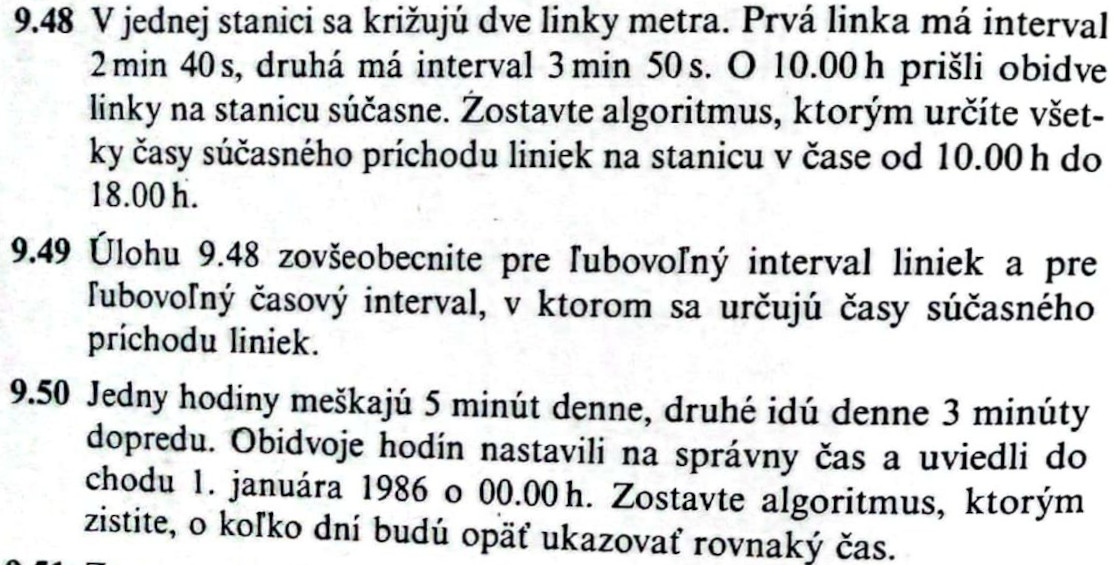
\includegraphics[width=0.9\textwidth]{assets/zbierka-mat-cyklus.jpg}}
\caption{Úlohy na príkaz cyklu}
\end{subfigure}
\caption{Ukážky z kapitoly algoritmy v zbierke úloh z matematiky pre 3. ročník~SŠ}
\label{fig:matematika-slovne-ulohy}
\end{figure}

Odlišný prístup ku grafickej úprave majú knihy zo série ,,Skúsiš to s ...'', v rámci ktorej boli uvedené knihy programovania pre mikropočítače v Basicu a strojovom kóde (\cite{tatchellova_skusis_1990}, \cite{wattsova_skusis_1991}). Cieľové miesta pôsobenia knihy neboli v čase vydania zrejme školy, ale skôr počítačové krúžky ako voľnočasové aktivity. Tieto dve knihy sa nápadite odlišujú pestrofarebnými ilustráciami až takmer komiksovým podtónom, kde sú hlavnými hrdinami roboti v ľudskom a hmyzom stvárnení a mimozemšťania. Krátke odseky výkladového textu sú obohatené o motivovanie každého príkazu jednoduchým príkladom priamo pobádajúcim na odskúšanie (Obr.~\ref{fig:skusis-prog-premenne}). Funkčné bloky kódu rozsiahlejších programov sú priebežne vysveľované textom so svorkami (Obr.~\ref{fig:skusis-prog-kozmicke-bane}), čo môže slúžiť ako dobrý model na prezentovanie riešení v zbierke.

\begin{figure}[h]
\centering
\begin{subfigure}[b]{0.55\textwidth}
\centering
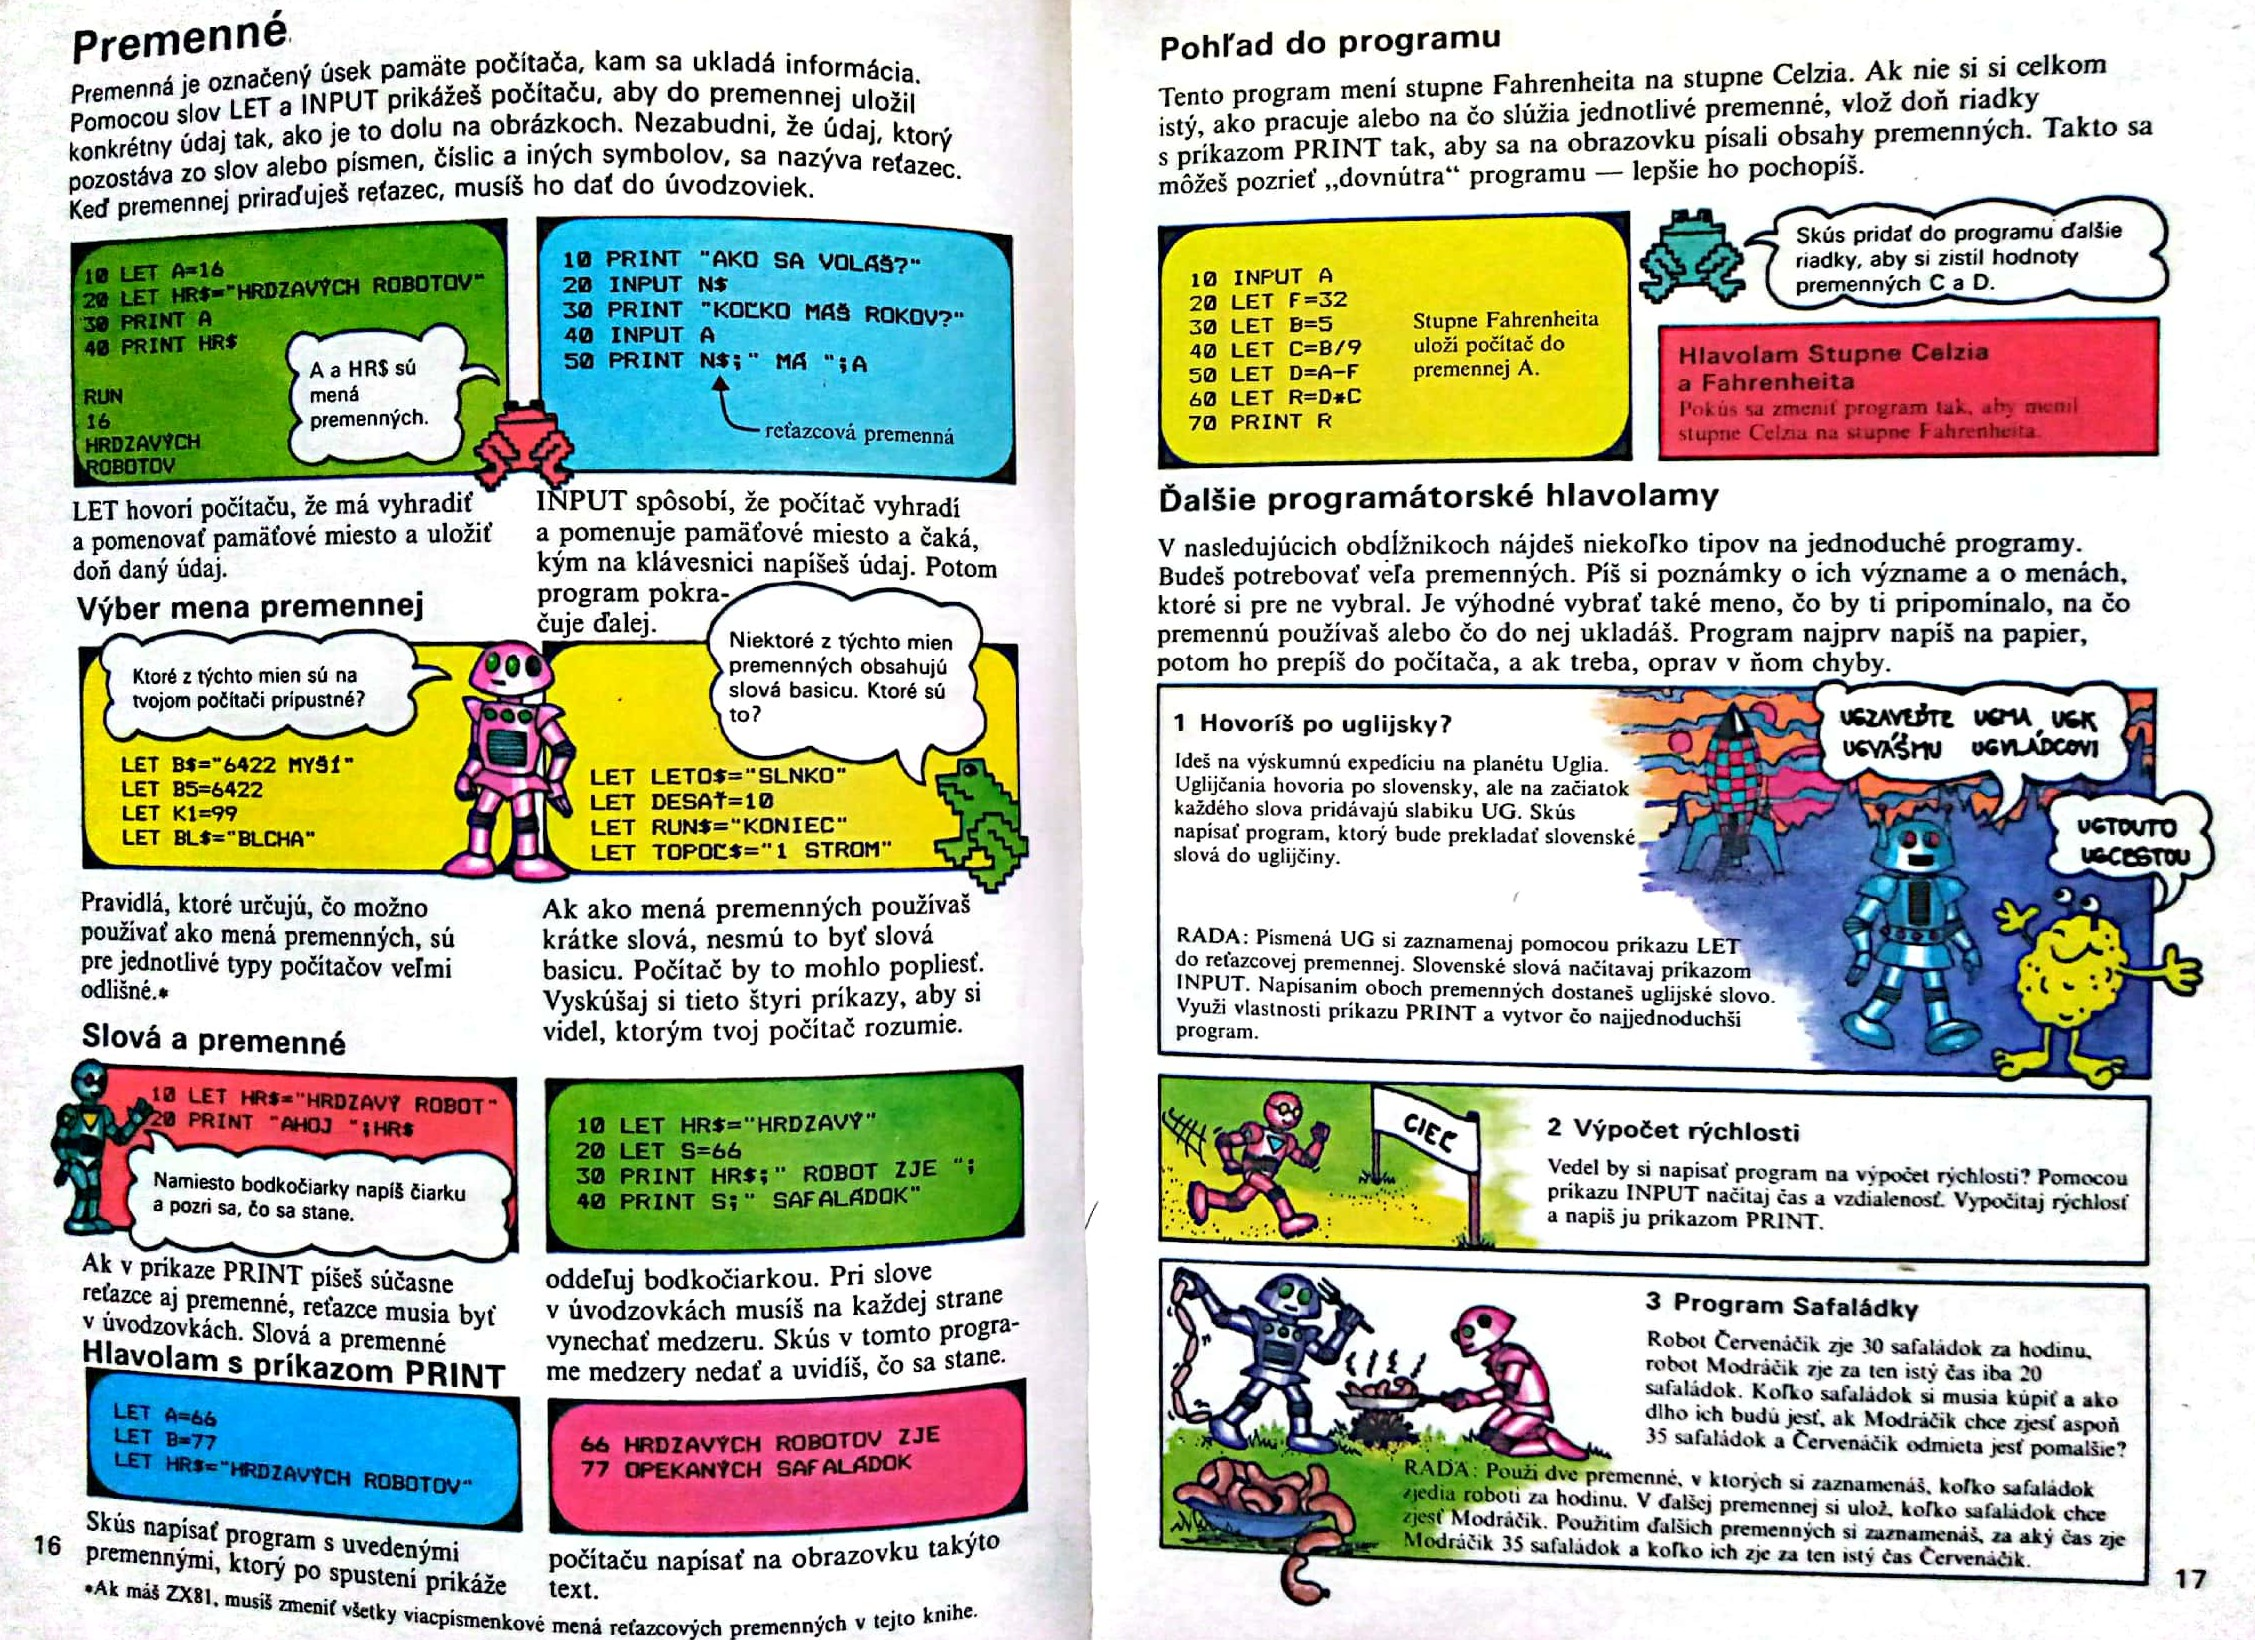
\includegraphics[width=\textwidth]{assets/kniha-premenne.jpg}
\caption{Výkladový text o premenných s hlavolamami}
\label{fig:skusis-prog-premenne}
\end{subfigure}
\hfill
\begin{subfigure}[b]{0.44\textwidth}
\centering
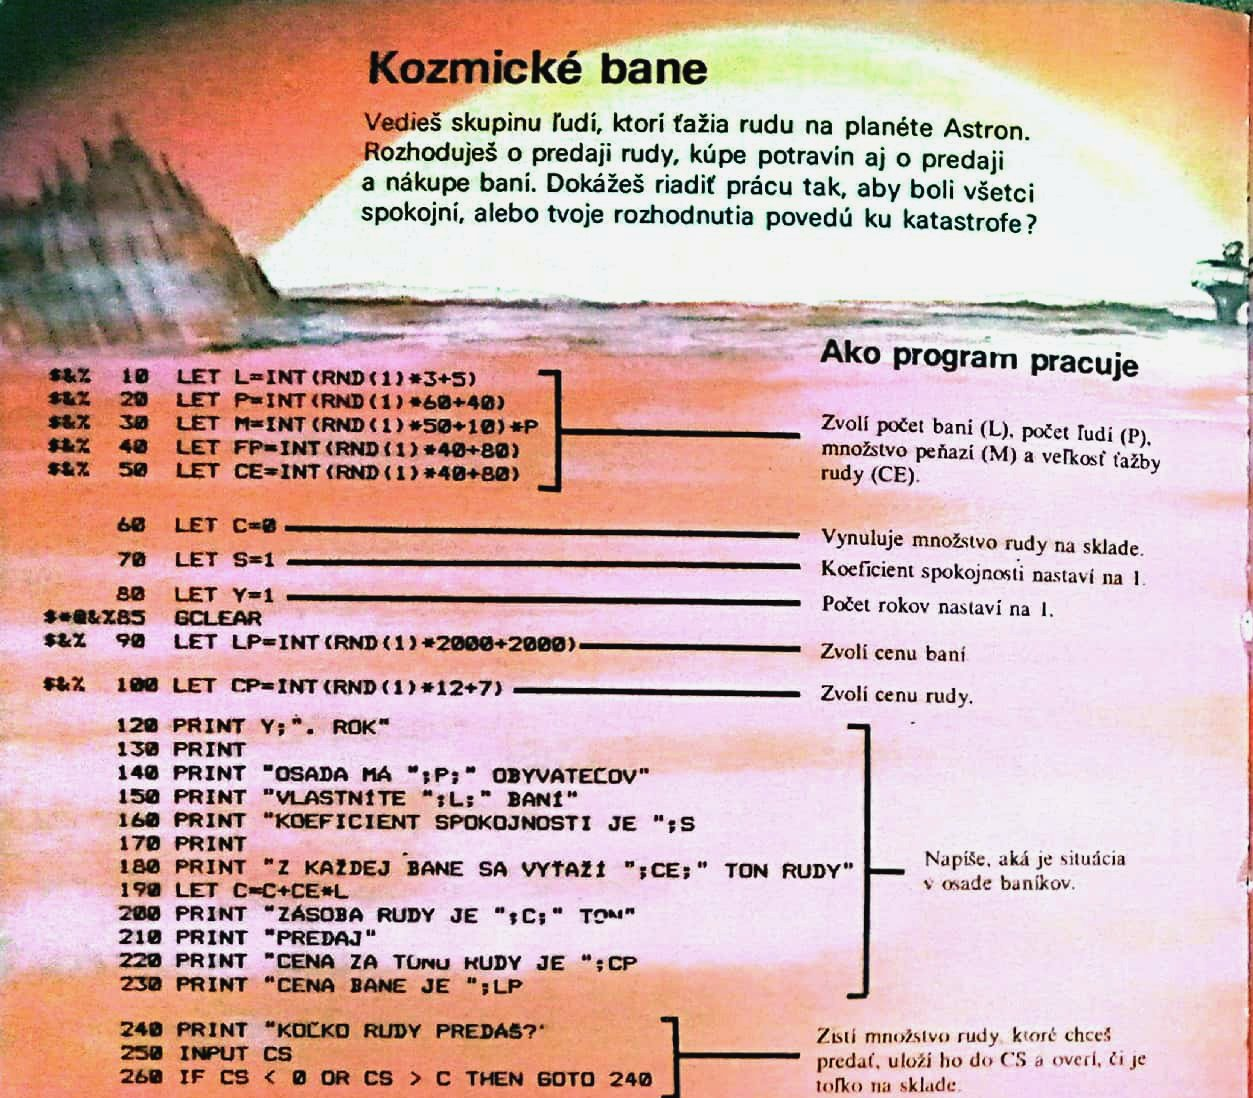
\includegraphics[width=\textwidth]{assets/program-kozmicke-bane.jpg}
\caption{Opis kódu program počítačovej hry}
\label{fig:skusis-prog-kozmicke-bane}
\end{subfigure}
\caption{Bohato ilustrovaná kniha o programovaní v jazyku Basic}
\end{figure}

Učebné texty na webe pod názvom: ,,Algoritmy a programovanie v Pascale: nielen pre maturantov z predmetu informatika'', tvoria obsiahly prierez prvkov programovacieho jazyka konkrétne: výraz s premennou, údajové typy, vetvenie, cyklus, cyklus v cykle, procedúry, funkcie, rekurzia, jednorozmerné polia, textový súbor, vyhľadávanie a triedenie polí, reťazce znakov (\cite{hedvigova_algoritmy_2007}). Učebnica je prehľadne štruktúrovaná. Z obsahu sa hypertextom smeruje na kapitoly, kde je každý nový pojem typograficky zvýraznený podčiarknutím, príkazy jazyka sú odlíšené neproporcionálnym rezom a farbou písma. Po jadre kapitoly nasledujú obvykle 2 vzorové príklady s riešeniami, spravidla 3 priebežné programátorské úlohy (Obr.~\ref{fig:uloha-pascal}), otázky na opakovanie teórie, a úlohy na precvičovanie celej témy. Na konci učebnice je umiestnených 51 jednoduchších úloh na opakovanie a 30 úloh pre náročnejších, ktorým však chýba zmysluplná organizácia náročnosti.

\begin{figure}[h]
\centering
\fbox{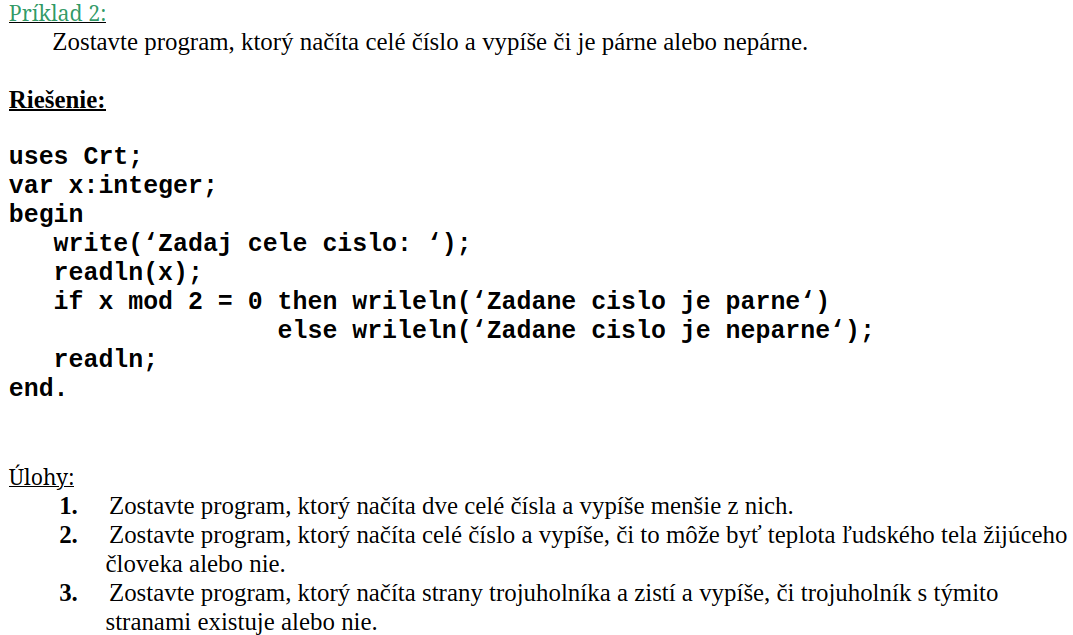
\includegraphics[width=0.8\textwidth]{assets/uloha-pascal.png}}
\caption{Riešený príklad z vetvenia nasledovaný úlohami na samostatnú prácu}
\label{fig:uloha-pascal}
\end{figure}

Slovné úlohy objasňujúci s príbehom  problémové situácie, sú prítomné v súťažiach ako sú Olympiáda v Informatike, organizovanú Národným inštitútom vzdelávania a mládeže, alebo Zenit, Korešpondenčný seminár (KSP) a Letné školy, organizované občianskym združením Trojsten. Vzorové riešenia zadaní vychádzajú v príručkách po skončení kôl. Keďže úlohy bývajú nad rámec základného učiva, tak na vysvetlenie často sa vyskytujúcich algoritmov vznikla tzv. Kuchárka KSP (\cite{noauthor_kucharka_2022}). Ukážka na Obr.~\ref{fig:ksp-oblecenie} ilustruje predlohu pre zadanie z KSP, ktorá sa vyznačuje okrem popisu situácie cez krátky dej, jasným stanovením vstupov a výstupov. 

\begin{figure}[h]
\centering
\fbox{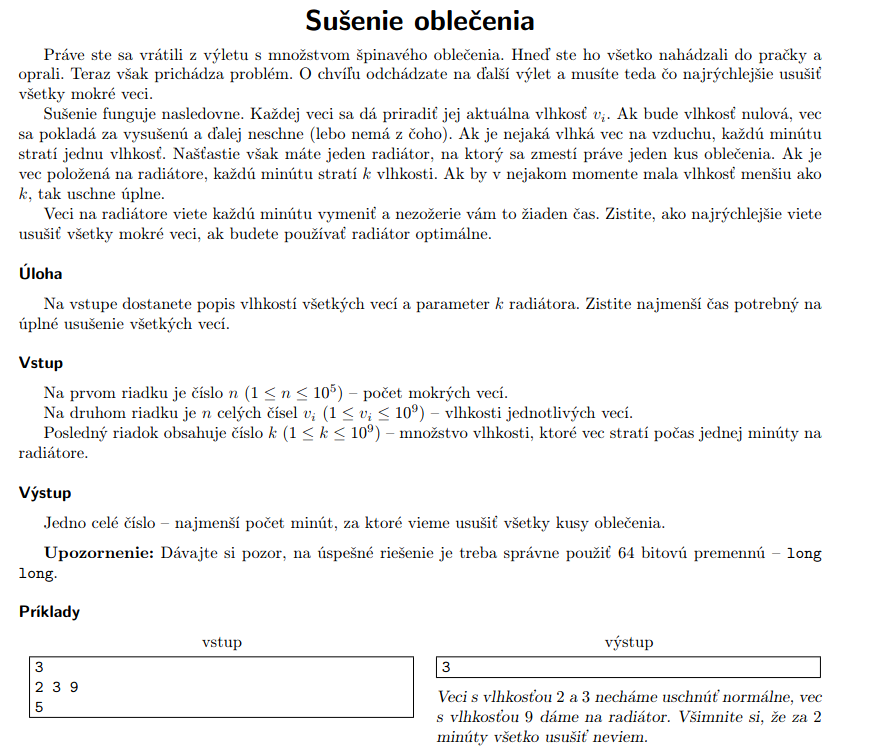
\includegraphics[width=0.8\textwidth]{assets/susenie-oblecenia.png}}
\caption{Úloha letnej školy KSP na binárne vyhľadávanie s úvodným príbehom}
\label{fig:ksp-oblecenie}
\end{figure}

Uvedenie programovacieho jazyka \emph{Python} do výučby informatiky na stredných školách znamenal dopyt po nových učebných materiáloch, ktoré preložia zápisy hlavne z dosiaľ používaného jazyku Pascal. Populatitu nadobudol Python vďaka odstráneniu deklarácie typu premenných a čitateľnejšiemu zápisu, pretože odsadením nahrádza označenie blokov kľúčovými slovami (\emph{begin} a \emph{end}) alebo zloženými zátvorkami. Medzi učebnicami Pythonu prevláda trend predstavovať programovanie cez procedurálne kreslenie cez modul \emph{tkinter}, \emph{turtle}, niekedy \emph{pygame}. V grafickom programovaní sa pojem cyklu prestavuje oveľa skorej ako podmienky, presne naopak než v textovom móde.

Kučera a Výbošťok dali dohromady trojdielnu sériu učebníc ,,Programujeme v Pythone'', v slovenskom a anglickom jazyku so zodpovedajúcimi príručkami pre učiteľov a testami k učebnici. Vypracovali aj zbierku 64 riešených úloh k maturite z informatiky ,,Maturujeme v Pythone''. Vychádzali z potrieb aktívnych učiteľov z Klubu učiteľov vedeného autorom. Osnova prvého diela učebnice začína grafickými príkazmi (Obr.~\ref{fig:kucera-kreslenie-python}) a ďalej sa skladá z premenných, opakovaní častí programu, podprogramov, klikania myšou a ovládaním klávesnicou, podmienených príkazov, časovača a snaženie sa zavŕši tvorbou jednoduchých hier (\cite{kucera_programujeme_2016}). 

\begin{figure}[h]
\centering
\begin{subfigure}[b]{0.55\textwidth}
\centering
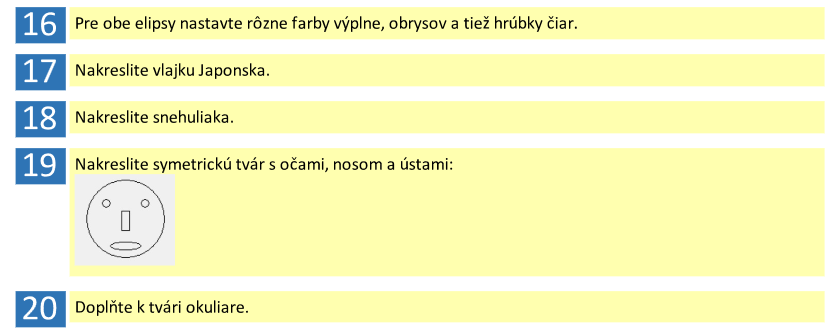
\includegraphics[width=\textwidth]{assets/kucera-python.png}
\caption{Kreslenie obdĺžníkov}
\label{fig:kucera-kreslenie-python}
\end{subfigure}
\begin{subfigure}[b]{0.44\textwidth}
\centering
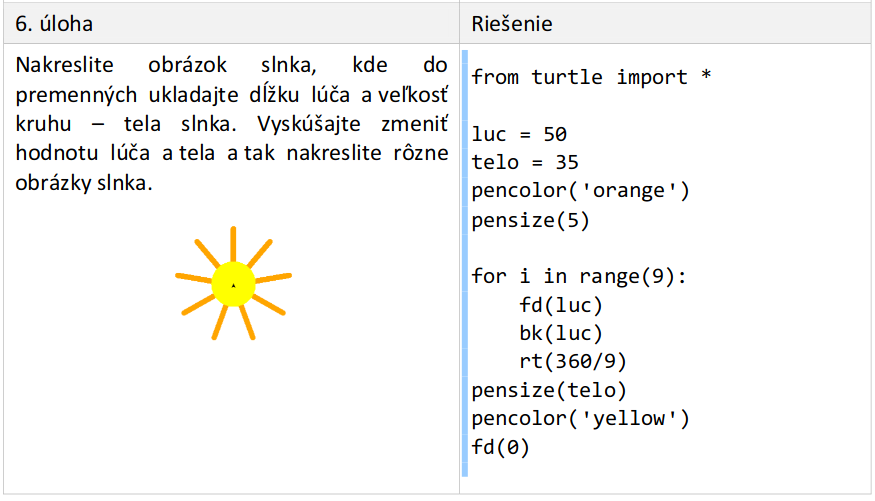
\includegraphics[width=\textwidth]{assets/uloha-turtle.png}
\caption{Cyklus a korytnačia grafika}
\label{fig:turtle-graphics}
\end{subfigure}
\caption{Úlohy na programovanie grafiky v jazyku Python}
\end{figure}

Blaho a Salanci pripravili pracovné listy \emph{abcPython} na 20 vyučovacích hodín, kde nepočítajú s výkladom učiteľa. Dostupné sú aj metodické materiály ku listom. Preberajú sa postupne témy kde sa prelína textový a grafický režim: interaktívny zadávanie príkazov, výrazy, premenné, výpisy, kreslenie, náhoda, výrazy v cykle, elipsy, vetvenie, podprogramy, kreslenie myšou (\cite{blaho_abcpython_2019}, \cite{blaho_metodiky_2019}). 

Mészárosová vytvorila metodickú príručku pre vyučovanie základov programovania, kde cez Python rozvíja na rozpätí 16 vyučovacích hodín korytnačiu grafiku (Obr.~\ref{fig:turtle-graphics}). Využíva tým oboznámenosť žiakov s korytnačkami v jazyku Logo z druhého stupňa základnej školy. Rovnako sa začína predstavením grafickými pokynov na pohyb a kreslenie korytnačkou. Nasledujú premenné, for cyklus, funkcie, funkcie s parametrami, poloha korytnačky, náhodná poloha, vetvenie a na upevnenie zručností slúži projekt kreslenia pohľadnice (\cite{meszarosova_python_2017}).



\chapter{Cieľ a metodika práce}
Cieľom záverečnej práce je zostaviť rozšíriteľnú \textbf{zbierku úloh z programovania} so vzorovými riešeniami v predmete informatika pre stredné školy. Primárny zámer súčasne vyžaduje uspokojenie nasledujúcich požiadaviek na navrhnutý systém úloh pre pedagogickú prax:

\begin{itemize}[noitemsep]
\item pokrytie základného učiva v súlade so ŠVP a cieľovými požiadavkami
\item poskytnutie metodiky na spôsob zaradenia ďalších úloh do nášho systému úloh
\item čitateľnosti textu zadaní primeranej žiakom vo veku 15 - 18 rokov
\item príbehovosť opisu problémovej situácie v znení zadania
\item vzorové riešenia v programovacom jazyku Python
\item zobrazenie na webovej stránke s efektívnym využitím hypertextu
\end{itemize}

Splnenie vytýčených cieľov sa opiera o rešerš informačných zdrojov vyhľadaných prostredníctvom plnotextových vyhľadávačov webu a knižníc, na základe rád školiteľky a osobného povedomia o oblasti. Knihy a články boli podrobené procesu analýzy, kedy sa vyselektovali relevantné definície, charakteristiky, kategorizácie a postupy. Metóde porovnania sa podrobili existujúce učebné texty základov programovania.

Vlastná tvorba zbierky úloh prebiehala syntézou psychologických východísk porozumenia textu, známych typových úloh a známej metodiky na preformulovanie úloh. Hodnotenie kvality textu úloh v zbierke sa uskutočnilo kvantitatívne i kvalitatívne. Úroveň čitateľnosti sa indikatívne vyčíslila pomocou Gunning fog indexu (Vzorec~\ref{equ:fog-index}). Kvalitatívne sa pozorovali problémy  žiakov pri riešenia úloh v zbierke na vyučovacej hodine plynúcej z neporozumenia formulácie zadania. Metodika klasifikácie úlohy v systéme vychádza z kritérií témy, podtémy, elementu, didaktickej funkcie a kognitívnej úrovne podľa Minďákovej (Sekcia~\ref{sec:klasifikacia-ulohy}).


\chapter{Metodika práce a metódy skúmania}
        (11) Časť Metodika práce a metódy skúmania spravidla obsahuje:
            a) charakteristiku objektu skúmania, 
            b) pracovné postupy, 
            c) spôsob získavania údajov a ich zdroje, 
            d) použité metódy vyhodnotenia a interpretácie výsledkov,
            e) štatistické metódy. 

 


\chapter{Výsledky práce}
Výsledky práce a diskusia sú najvýznamnejšími časťami záverečnej práce. Výsledky (vlastné postoje alebo vlastné riešenie vecných problémov), ku ktorým autor dospel, sa musia logicky usporiadať a pri popisovaní sa musia dostatočne zhodnotiť. Zároveň sa komentujú všetky skutočnosti a poznatky v konfrontácii s výsledkami iných autorov. Ak je to vhodné, výsledky práce a diskusia môžu tvoriť aj jednu samostatnú časť a spoločne tvoria spravidla 30 až 40 \% záverečnej práce.

\section{Zbierka úloh}

1. Premenné - 13 úloh
2. Podmienky - 7 úloh
3. Cykly - 9 úloh
4. Náhodné čísla - 3 úlohy
5. Zoznamy - 9 úloh
6. Súbory - 6 úloh
7. Funkcie - 11 úloh

\subsection{Predhovor}
\setlength\epigraphwidth{12cm}
\setlength\epigraphrule{0pt}
\epigraph{\small\itshape Umenie programátora je najmä o schopnosti meniť úrovne abstrakcie, z nízkej na vysokú úroveň. Niečo vidieť v malej a niečo vidieť vo veľkej mierke.}{--- \textup{Donald Knuth}}

Každý je raz na začiatku a stojí pred výzvou ako zvládnuť kostrbatú cestu, ktorá ho čaká.  Programovanie nie je v tomto ohľade výnimkou. Vedieť požiadať neživý predmet, počítač, aby  spravil to, čo od neho chceme, stojí nemalé úsilie. Často sa pri tom zasekneme na rôznych  chybách objavujúcich sa medzi zadaním a riešením problému. 

Zo začiatku si prejdeme cez množstvo vzájomných nedorozumení. Rečou stroja sú totiž mystické  postupnosti binárnych čísel. Ľudia našťastie vymysleli programovacíe jazyky, vďaka ktorým sa  dokážeme lepšie pochopiť. Naučiť sa plynulo rozprávať s týmto cudzincom si aj napriek tomu  vyžaduje veľa času a hlavne neustáleho prekonávania nových výziev.

Táto zbierka úloh si kladie za cieľ byť tvojim spoločníkom pralesom kódu od prvých pozdravov až k rozsiahlym esejám. Krása textov nebude spočívať v rýmoch básne, ale v presnej a usporiadanej logickej štruktúre. Naša činnosť bude podobná kuchárovi, keď objaví chutnú kombináciu prísad. Dá ich dokopy presným postupom a následne svoje majstrovstvo premení do receptu, aby si nové unikátne jedlo mohli uvariť a vychutnať všetci.

Pri ochutnávke sveta softvéru prejdeme od priamej postupnosti príkazov, cez rozhodnutia spracovania viacerých údajov v cykloch, až po využívanie súborov na ukladanie celých databáz. Našimi prísadami budú dáta a postupom algoritmy, alebo teda programy. Nezaháľajme teda a vydajme sa na púť.

\subsection{Premenné (\rom{1}.)}
\textbf{Premenná} je ako krabička slúžiaca na odkladanie informácií, ktoré si potrebujeme pre vykonanie danej činnosti zapamätať. Podľa účelu sa líšia svojim *dátovým typom*, ktorý sa vytvorí, keď do premennej niečo vložíme (*priradenie*) a určuje to, čo sa vo vnútri nachádza.

Základné stavebné kamene, z ktorých vyskladáme opis zložitejších javov sú:

\begin{itemize}
\itemsep0pt
\item \textbf{Logická hodnota} (\textit{bool}) - Boolean môže mať len dve hodnoty - pravda (\textit{True}) alebo nepravda (\textit{False})
\item \textbf{Celé číslo} (\textit{int}) - Do integer-u ukladáme ľubovolné kladné a záporné celé čísla (napr. \textit{97})
\item \textbf{Desatinné číslo} (\textit{float}) - Líšia sa od celých čísel spôsobom uloženia (napr. \textit{3.14159})
\item \textbf{Reťazec} (\textit{str}) - Označujeme ich úvodzovkami alebo apostrofmi a väčšinou predstavujú text napísaný na klávesnici alebo zobrazený na obrazovke. (napr. \textit{"Učím sa programovať!"})
\end{itemize}

\subsubsection*{1. Pozdrav}
Vytvor program, ktorý ťa po vložení mena pozdraví. Zameň pozdrav a zároveň nechaj program sa rozlučiť.

\begin{code}
Ako sa voláš?: ______
Ahoj ______
\end{code}

\subsubsection*{2. Básnik}
Vytváraš básničky na počkanie. Dnes sa ti ťažko premýšľa nad kreatívnymi textami, tak si chceš ušetriť námahu tým, že budeš meniť len rým.

\begin{code}
Napíš slovo, ktoré sa rýmuje so slovom strach: _____
Tu je báseň:
Z počítačov mával som vždy strach
teraz som však šťastný ako _____.
\end{code}

\subsubsection*{3. Pozvánka}
Každému kamarátovi chceš poslať pozvánku na svoju narodeninovú oslavu. Okrem mena v správe potrebuješ meniť aj čas konania oslavy (nie všetci chodia načas), vec, ktorú priniesie a jedlo, ktoré bude mať prichystané.

\begin{code}
Meno kamaráta: _____
Čas oslavy: _____
Prines: _____
Jedlo: ______

Ahoj _____,
pozývam ťa na moju narodeninovú oslavu, ktorá sa bude konať 12.4. o _____. Nezabudni priniesť _____ a pekný darček. Na večeru ťa čaká _____ a samozrejme lahodná torta. Teším sa na teba! :)
\end{code}

\subsubsection*{4. Prevod jednotiek teploty}
Prišiel si na návštevu v Amerike a keď ideš von nevieš ako sa máš obliecť, lebo na teplomere vidíš len stupne Fahrenheita ($F$). Premeň ich na stupne Celzia ($C$).

$$ C = (F - 32) \cdot (5 / 9) $$

\begin{code}
Vonku je °F: _____
Doma by to bolo _____°C.
\end{code}

\subsubsection*{5. Hlboká roklina}
Stojíš na útese nad hlbokým údolím a rozmýšlaš ako odmerať jej hĺbku (*h*). Vtom ťa osvietia tvoje dávne vedomosti z fyziky. Zoberieš do ruky kameň a pustíš ho z ruky do rokliny.
Zároveň spustíš stopky a zmeriaš čas dopadu. Rýchlosť zvuku rachotu pri náraze na zem môžeme zanedbať. Na kameň sa ohybuje sa nadol rovnomerným spomaleným pohybom. Pôsobí naň tiažové zrýchlenie: $g = 9.81$.
$$ h = (gt^2)\;/\; 2 $$

\begin{code}
Čas dopadu kameňa (s): ________
Hĺbka rokliny je potom _______ metrov.
\end{code}

\subsubsection*{6. Vedro s vodou}
Do nádrže z dažďovou vodou napršalo cez noc veľa vody. Jediný spôsob ako zúžitkovať zachytenú vodu je preniesť ju vo vedre valcového tvaru. Naberieme vždy len toľko vody koľko budeme potrebovať, preto je dobré poznať objem vedra. Rozmery vedra dokážeme odmerať pravítkom. Objem valcového vedra $V$ s výškou $v$ a priemerom podstavy $d$ sa vypočíta ako:
$$ V = \pi \cdot (d\;/\;2)^2 \cdot v $$

\begin{code}
Výška vedra (cm): ________
Priemer dna (cm): ________

Do vedra sa zmestí _______ litrov vody.
\end{code}

\subsubsection*{7. Cesta autom}
Plánuješ trasu na výlet autom a chceš zistiť akou rýchlosťou musíte priemerne ísť, aby ste stihli navštíviť všetky miesta a prišli večer včas do hotela.

\begin{code}
Dĺžka cesty (km): ____
Odchod z domu (hodina): ____
Príchod do hotela (hodina): ____

Pôjdete priemerne ____ km/h.
\end{code}

\subsubsection*{8. Kúpalisko}
Začína sa letná sezóna a prevádzka kúpaliska musí pred otvorením plne napustiť bazény v areáli. Všetky sú kvádrového tvaru a poznáme ich rozmery. Zaujíma nás spotrebovaná voda na konkrétny bazén a cena, ktorú za ňu zaplatíme.

\begin{code}
Dĺžka bazéna (m): ____
Šírka bazéna (m): ____
Hĺbka bazéna (m): ____
Hĺbka hladiny od okraja (cm): ____
Cena za m^3 vody v eurách: _____

Na bazén sa minie ____ litrov vody a bude to stáť ____ eur.
\end{code}

\subsubsection*{9. Maľovanie}
Sťahuješ sa s rodičmi do nového bytu a dali ti za úlohu vymalovať si izbu. Myslíš si, že nástroj na rýchle počítanie množstva farby by sa hodil aj profesionálnym maliarom, preto vytvoríš program na vypočítanie plochy stien a stropu bez okna a podlahy.

\begin{code}
Rozmery miestnosti
Dĺžka (cm): ____
Šírka (cm): ____
Výška (cm): ____
Rozmery okna
Šírka (cm): ____
Výška (cm): ____
Výdatnosť farby (m^2/kg): ____

Maľovať budeš plochu ____ m^2. Kúp ____ kg farby.
\end{code}

\subsubsection*{11. Pokladnička}
Do banky vložíme peniaze (vklad)  a každý rok sa nám na nich pripočítava úrok. V banke necháme peniaze určitý počet rokov. Vypočítajte ako sumu dostaneme pri výbere.

Napíš program, ktorý nám umožní na vstupe napísať rôzne sumy peňazí, úrokové miery a obdobie sporenia a na výstupe vypíše nasporenú sumu. Vyberte si, či použijete jednoduché alebo zložené úročenie - vzorec nájdite na internete alebo v zošite matematiky. Spustenie programu môže vyzerať nasledovne (pri jednoduchom úročení):

\begin{code}
Vklad (euro): ____
Úrok (%): ___
Dĺžka sporenia (rok): ___

Na konci sporenia si v banke vyberieš _____ eur.
\end{code}

\subsubsection*{12. Chemikálie}
Napíš program na výpočet zmiešavania dvoch roztokov. Každý roztok je opísaný svojou hmotnosťou ($m$) v gramoch a hmotnostným zlomkom rozpustenej látky v rozpúštadle ($w$) v percentách.
 
Roztoky vo vzorci sú rozlíšené dolným indexom, napr. . Na vstupe sú zadané všetky premenné s indexami 1 a 2. Premenné s indexom 3 je potrebné vypočítať v programe.  Percentá je potrebné prerátať na pomer z celku vydelením 
100-mi.

Na výpočet v programe využiješ rovnice:
$$m_3 = m_1 + m_2$$
$$m_3 \cdot w_3 = m_1 \cdot w_1 +  m_2 \cdot w_2$$

\begin{code}
m1 (hmotnosť roztoku č.1)? ___
w1 (hmotnostný zlomok roztoku č.1)? ___
m2 (hmotnosť roztoku č.2)? ___
w2 (hmotnostný zlomok roztoku č.2)? ___

Výsledný roztok má hmotnosť ___ g.
Hmotnostný zlomok rozpustenej látky je ___ %.
\end{code}


\subsubsection*{13. Brzdenie}
V poslednej dobe je na trati viacej nebezpečných zrážok. Rušňovodiči ťa požiadali, aby si zistil ako rýchlo pred prekážkou dokáže vlaková súprava zastaviť pri danej rýchlosti.

\begin{itemize}
\itemsep0pt
\item Kinetická energia pohybujúceho sa vlaku (práca potrebná na zabrzdenie): $ W = E_k = \frac{1}{2} \cdot m \cdot v^2 $
\item Brzdná dráha pri brzdnej sile $F_b$: $ s = \frac{W}{F_b \cdot m} $
\item Čas potrebný na zastavenie vlaku pri rovnomernom spmalenom pohybe: $ t = \sqrt{\frac{2 \cdot s}{F / m}} $
\end{itemize}

\begin{code}
Vlaková súprava
- Rýchlosť (km/h): ____
- Hmotnosť lokomotívy (t): ____
- Hmotnosť vagóna (t): ____
- Počet vagónov: ____
- Počet miest na vagón: ____
- Zaplnenosť vlaku (%): ____
- Brzdná sila (N/t): ____

V rýchlosti ____ km/h zabrzdí súprava s hmotnosťou ____ t na vzdialnosť _____ m a bude to trvať ____ s.
\end{code}


\subsection{Podmienky (\rom{2}.)}
\textbf{Podmienky} sú ako križovatky na ceste. Podľa toho kam chceme ísť, sa rozhodneme, ktorou cestou pôjdeme ďalej. Aby sme sa uistili, že máme ten správny smer (*vetva podmienky*) pýtame sa vždy logickú otázku pomocou už získaných údajov uložených v premenných.

\subsubsection*{1. Heslo}
Tvoj dom na strome už vykradlo pár nezvaných návštevníkov a preto si vymyslel spôsob ako dovoliť návštevu len povoleným osobám, ktoré poznajú tajné heslo.

\begin{code}
Stoj! Povedz Heslo!
> _____

Vstúp, priateľ /   Zmizni kade ľahšie
\end{code}


\subsubsection*{2. Najväčšie číslo}
Zisti, ktoré z troch zadaných čísel je najväčšie.

\begin{code}
1.číslo: ____
2.číslo: ____
3.číslo: ____

Najväčie je ____.číslo a to je ____.
\end{code}


\subsubsection*{3. Vhodné oblečenie}
Módni poradcovia vyšli z módy a ich prácu prebrali počítače. Na základe počasia a príležitosti odporúčajú vhodný outfit. Vymysli pár tipov pre rôzne situácie a začni radiť.

\begin{code}
Ako je vonku?: _____
Kam ideš?: ____

Určite si nezabudni _______ a tiež si vezmi _______.
\end{code}


\subsubsection*{4. Pokazený rozpis}
Podnik spracujúci rudu dostal časový rozpis trvania jednotlivých krokov vylepšeného technologického procesu. Činnosti zvyčajne trvajú dlhšie ako hodinu, nehodí sa im teda mať časy napísané iba ako údaj v minútach. Tvojou úlohou je rozpísať minúty na dni, hodiny, minúty pre jednoduchšie čítanie rozpisu. Vynechajte nepotrebné časové údaje.

\begin{code}
Trvanie (min.): ____
= ___ d. ____ hod. ___ min
\end{code}


\subsubsection*{5. Hovoriaca kalkulačka}
Výpočty neboli nikdy väčšia zábava, teda aspoň s kalkulačkou, ktorá namiesto čudných matematických znamienok hovorí ľudskou rečou. Vytvorte kalkulačku, ktorá si vypýta dve čísla a vie ich sčítať alebo odčítať.

\begin{code}
Som hovorica kalkulačka a rada počítam!
Povedz mi prvé číslo: ____
Potrebujem ďašie číslo: ____
Chceš ich sčítať alebo odčítať: ____ (sčítať / odčítať)

Výsledok tvojho príkladu: ____ plus/mínus _____ je ________.
\end{code}

\subsubsection*{6. Kvadratická rovnica}
Pre zadané koeficienty $a$, $b$, $c$ kvadratickej rovnice $ax^2 + bx + c = 0$  vypočítajte jej korene v obore reálnych čísel a vrchol paraboly daného predpisu.

\begin{code}
a = ____
b = ____
c = ____

___x^2 + ___x + ___ = 0
x1 = ____
x2 = ____
V[___; ___]
\end{code}

\subsubsection*{7. Trojuholníky}
Mýtická bytosť stredoškolskej matematiky, o ktorej je vždy treba zistiť, čo najviac bez rysovania, aj keď chýbajú rozmery.

\begin{enumerate}[label=\alph*)]
\item Ak je možné, doplň chýbajúce informácie pre ľubovoľný trojuholník (zadaný ako SSS) ako sú dĺžky strán a výšok, veľkosti uhlov, obsah a obvod. Využite trojuholníkoú nerovnosť, sínus(ovú) vetu, kosínus(ovú) vetu a vzorec na výpočet obsahu trojuholníkov.
\item Rozšírte vypočet aj pre ostatné vety o trojuholníkoch: SUS, USU, UUS
\end{enumerate}

\begin{code}
Zadajte strany ľubovolného trojuholníka:
a = ___
b = ___
c = ___

Strany: a = ___; b = ___; c = ___
Uhly: alpha = ___°; beta = ___°; gamma = ___°
Výšky: v(a) = ___; v(b) = ___; v(c) = ___
O = ___
S = ___
Trojuholník je: ____, _____
\end{code}


\subsection{Cykly (\rom{3}.)}
Obrovský potenciál počítačov tkvie v bezchybnom neúnavnom vykonávaní presne zadaných inštrukcií. Cykly umožňujú opakovať rovnaký postup ľubovoľný počet krát a tým efektívne odstraňovať rutinnú prácu.


\subsubsection*{1. 100-krát napíš}
Za vyrušovanie na hodinách sa stalo populárnym trestom ručné prepisovanie mravoučnej vety stokrát. Stalo sa to tak neznesiteľné, že si zhotovil robota, ktorý vie pomocť záškodníkom. Chýbajú mu len príkazy, čo má vlastne robiť.

\begin{code}
Musím napísať: _____
Toľkoto krát: ____

______
______
...
\end{code}


\subsubsection*{2. Hodnotenie}
Filmový kritici a hodnotitelia reštauracií zapíšu po namáhavom dni číselné skóre k ich recenziam. Pre lepší efekt potrebujú vykresliť hviezdničky namiesto čísla. Pomôž im.

\begin{code}
Skóre: 5

*****
\end{code}

\subsubsection*{3. Pyramída}
Hviezdičky zoskup do tvaru pyramídy zadanej výšky.

\begin{code}
Výška pyramídy: 4

   *
  ***
 *****
*******
\end{code}

\subsubsection*{4. Smaragd}
Na pyramídu pripoj zo spodu ďaľšiu obrátene, aby vznikol smaragd z hviezdičiek.

\begin{code}
Veľkosť: 5

  *
 ***
*****
 ***
  *
\end{code}

\subsubsection*{5. Duté vnútro}
Nakresli duté pyramídu a smaragd podľa prechádzajúcich úloh.

\begin{code}
Výška pyramídy: 4

    *
   * *
  *   *
 *******
\end{code}


\subsubsection*{6. Mriežka slov}
Načítajte veľkosť tabuľky a slovo, ktoré sa v nej bude na každom riadku v stĺpci opakovať.

\begin{code}
Počet riakov a stĺpcov: 4
Opakovať slovo: ano

ano ano ano ano
ano ano ano ano
ano ano ano ano
ano ano ano ano
\end{code}



\subsubsection*{7. Rám}
Prvý a posledný riadok a stĺpec bude tvoriť rám pre mriežku slov.

\begin{code}
Počet riakov a stĺpcov: 4
Opakovať slovo: ano

### ### ### ###
### ano ano ###
### ano ano ###
### ### ### ###
\end{code}


\subsubsection*{8. Malá násobilka}
K výbave každého žiaka základnej školy patrí tabuľky malej násobilky. Vytvor takúto tabuľku obsahujúcu každý násobok od 1x1 po 10x10, aby si pomohol všetkým malým matematikom.

\begin{code}
   1   2   3   4   5   6   7   8   9  10
   2   4   6   8  10  12  14  16  18  20
   3   6   9  12  15  18  21  24  27  30
   4   8  12  16  20  24  28  32  36  40
   5  10  15  20  25  30  35  40  45  50
   6  12  18  24  30  36  42  48  54  60
   7  14  21  28  35  42  49  56  63  70
   8  16  24  32  40  48  56  64  72  80
   9  18  27  36  45  54  63  72  81  90
   10  20  30  40  50  60  70  80  90 100
\end{code}


\subsubsection*{9. Sporenie}
Na letnej brigáde si zarobil peniaze, ktoré chceš usporiť. Porovnáš ponuky bánk a hľadáš najvýhodnejší plán. Vytvor si sporiacu kalkulačku, ktorá na základe nemenného počiatčného vkladu, ročnej úrokovej sadzby, typu úročenia a žiadanej konečnej sumy, vypíše vývoj tvojich finančných prostriedkov do budúcnosti.

\begin{code}
Vklad v Eur: ____
Úroková sadzba p.a. v %: _____
Typ úročenia (jednoduché / zložené): _____
Žiadaná suma v Eur:

Rok      Suma         Úrok
  1.	     ______ Eur   _____ Eur
  2.     ______ Eur   _____ Eur
....
\end{code}



\subsection{Náhodné čísla (\rom{4}.)}
Pri tvorbe simulácií sú náhodné čísla nepostrádateľné. Umožňujú vniesť variabilitu a rôznorodosť do inak statických scén. Nesmierne poslúžia v hrách, kde dovoľujú modelovať napríklad pravdepodobnosť výskytu monštier, či pokladov.


\subsubsection*{1. Hádzanie kockou}
Vytvorte simuláciu hodu kockou. Po stlačení klávesy Enter sa nakreslí kocka s padnutým číslom.

\begin{code}
HOĎ<ENTER>
+-------+
| #   # |
|   #   |
| #   # |
+-------+
\end{code}

\subsubsection*{2. Hádaj číslo}
Náhodne vyber číslo s rozsahu medzi 0 a 100 a nechaj hráča hádať dokým neuhádne. Pri tom mu poskytni nápovedy, či je jeho tip priveľa alebo primalo. Zakomponuj rôzne obtiažnosti s možnosťou nastavenia rozsahu alebo maximálnym počtom tipov.

\begin{code}
Hádaj číslo: 8
Málo
Hádaj číslo: 18
Veľa
Hádaj číslo: 13
Výborne. Uhádol si!
\end{code}

\subsubsection*{3. Opakovanie násobilky}
Vďaka tvojej tabuľke malej násobilky sa malý školáci mohli naučiť násobiť. Ako dobre to vedia, musíš teraz odtestovať. Vygeneruj dve čísla od 1 do 10 do príkladu na násobenie. Over správnosť žiačikovej odpovede.

\begin{code}
Koľko je ____ x _____?
= _____
Správne - len tak ďalej / Nesprávne - hádaj znovu
Chceš ďalší príklad?
\end{code}


\subsection{Reťazce a zoznamy (\rom{5}.)}
\textbf{Zoznam} (tiež aj Pole) je množina údajov zaznamenaných spolu pod jedným menom. Každý údaj poľa sa nazýva *prvok* a poradie jeho pozície sa nazýva \textit{index}. \textbf{Reťazce} sa správajú podobne ako zoznamy, ale ich prvkami sú jednotlivé znaky.


\subsubsection*{1. Vymeň písmeno}
Niekto ti posiela správy s diakritikou, ale po ceste sa vždy prekrúti jedno písmeno. Texty obsahujú aj pekné básne, ktoré si chceš vytlačiť a pripnúť na nástenku. Pokazený znak však kazí celkový dojem z diela. Zameň zadané chybné písmeno v celom reťazci.

\begin{code}
Správa: ________
Za chybné písmeno: ____
Vymeň: ____

Opravené!
__________
\end{code}


\subsubsection*{2. Cenzúra}
Prišla tvrdá cenzúra s nariadením, že nikto už nesmie vidieť žiadnu samohlásku. Nahraď každý prečin vo vstupnom texte ľubovoľným iným špeciálnym znakom.

\begin{code}
Správa: Ja som tvoj kamarat
Samohlásku nahraď: *

Cenzurované: J* s*m tv*j k*m*r*t
\end{code}


\subsubsection*{3. Počítanie slov}
Do redakcie miestnych novín chodia denno denne články, vtipy, poviedky a príbehy zo života od verných čitateľov. Aby mohli byť uverejnené potrebujú sa zmestiť do vyhradeného priestoru. Vypíš počet znakov, slov, viet a normostrán (\textbf{1800 znakov}) pre rýchlejšie spracovanie textov.

\begin{code}
Článok: _________

Znaky: ___
Slová: ___
Vety: ___
Normostrany: ____
\end{code}


\subsubsection*{4. Najdlhšie slovo}
Hra staršia ako ľudstvo samo. Debatný spolok usporiadal súťaž o nájdenie najdlhšieho slova, ktoré sa kedy vyskytlo v historických prejavoch. Zaujali ťa odmeny, ale nechce sa ti prehrabávať knižnicou starých záznamníkov a preto si prácu uľahčíš. Nájdi najdlhšie slovo v reťazci.

\begin{code}
Rečnícky prejav: ________

Najdlhšie slovo v ňom: _____
\end{code}

\subsubsection*{5. Výskyt písmen}
Dlho do noci čítaš časopisy o umelej inteligencii a fascinuje ťa jej schopnosť rozprávať sa s človekom. Na vytvorenie viet na danú tému potrebuje mať prehľad o percentuálnom výskyte hlások v texte. Spočítaj a vypíš zoznam frekvencie písmen v reťazci.

\begin{code}
Článok: _______

A: 23.2 %
B: 11.5 %
C: 8.9 %
...
Z: 0.3 %
\end{code}


\subsubsection*{6. Histogram}
Pri svojom predchádzajúceho pokuse s početnosťou písmen si všimneš, že každé ďaľšie písmeno v zozname sa oveľa menej objavuje ako očakávaš. Vykresli hviezdičky namiesto počtu percent a over si tak svoje pozorovanie graficky.

\begin{code}
Článok: _______

A: ****
E: *******
I: ****
...
X: *
\end{code}


\subsubsection*{7. Nákupný košík}
Pri veľkých nákupoch sa často zíde prehľadný zoznam s tým, čo doma treba. Pýtaj si položky s ich cenami až kým sa nerozhodneš, že máš spísané všetko. Zobraz prehľadnú orámovanú tabuľku s údajmi podobne ako na pokladničom bločku (názov tovaru, DPH tovaru, cena tovaru s DPH, celková suma na zaplatenie).

\begin{code}
Čo kúpiť?: ______
Cena ______?: _______
....

+----------+--------+--------------+
| Tovar    |  DPH   |  Cena s DPH  |
+----------+--------+--------------+
| Chlieb   |  0,20e |      0,98e   |
+----------+--------+--------------+
|    ...   |  ...   |     ...      |
+----------+--------+--------------+
| CELKOM   |  0,20e |      0,98e   |
+----------+--------+--------------+
\end{code}

\subsubsection*{8. Akronym}
SMS-ky rapídne zdraželi a napadlo ti, že bude lepšie posielať slovné spojenia ako skratky. Zo zadaných slov vytvor akronym. Vezmi začiatočné písmená každého slova a vytvor skratku, ktorá bude pozostávať len z týchto písmen.

\begin{code}
Slovné spojenie: Slovenské národné divadlo
Skratka: SND
\end{code}


\subsubsection*{9. Veľa opakovania}
Roboti rozvážajúci pizzu po meste si zaznamenávajú zmenu smeru pre postupné vylepšovanie trás na lokality k častým zákazníkom. Keďže sa firme darí, prešli roboti už toľko, že sa im všetky záznamy o ich cestách nezmestia do pamäti. Všimneš si, že si značia každý krok a to vedie k častému opakovaniu. Nahraď postupnosť za sebou idúceho písmena, počtom výskytu a písmenom (\textit{Run-length encoding})

\begin{code}
Cesta robota: NNNNNNSSSSSSSSSSSWWWWNNN
Skomprimované: 6N11S4W3N
\end{code}


\subsection{Súbory (\rom{6}.)}
\textbf{Súbor} je zoskupením súvisiacich údajov, ktoré sú uložené na disku počítača. Oproti načítavaniu vstupu z klávesnice majú výhodu hlavne pri spracovaní a uchovaní veľkého množstva dát. Súbory sa dajú: \textit{vytvoriť} / \textit{vymazať}, \textit{otvoriť} / \textit{zatvoriť}, \textit{čítať} / \textit{zapisovať}. Podľa typu uchovávaných údajov (označované \textit{príponou}) súbory rozdeľujeme na:

\begin{itemize}
\itemsep0pt
\item \textbf{Textové súbory} - .txt, .csv, .html, .py
\item \textbf{Obrazové súbory} - .bmp, .png, .jpg, .gif, .svg, .pdf
\item \textbf{Zvukové súbory} - .wav, .mp3, .midi
\item \textbf{Video súbory} - .avi, .mp4, .mkv
\item \textbf{Spustiteľné súbory} - .exe, .elf
\end{itemize}

V tejto kapitole budeme pre jednoduchosť pracovať s textovými súbormi:

\subsubsection*{1. Prepisovanie}
Pri prepisovaní dlhých textov na vstup programu sa často mýliš a príde ti to zbytočne zdĺhavé. Načítaj články u zadaní z predchádajúcej kapitoly zo súboru, ktorého názov si na začiatku vypýtaš. Pri úlohe "veľa opakovania" ulož záznam o ceste robota do nového súboru.


\subsubsection*{2. Turistika}
Na víkend sa črtajú ideálne podmienky na horskú turistiku. Nenecháš nič na náhodu a pripravíš si detailný plán s výškovým profilom trasy. Na každých desať metrov trasy si do súboru poznačíš aktuálnu nadmorskú výšku. Zisti celkové stúpanie a klesanie počas celého výletu spolu s najvyššou a najnižšou nadmorskou výškou. Vypíš aj celkovú dĺžku túry v kilometroch a trvanie prechodu horami v hodinách.

\paragraph{Vzorový obsah súboru (trasa.txt):}

\begin{code}
348
351
362
369
376
379
384
395
401
396
383
381
367
361
\end{code}

\paragraph{Turistika:}

\begin{code}
Výškový profil trasy je v súbore: ______

Trasa: 0.140 km - 0 h 21 min
Stúpanie: 53 m
Klesanie: 40 m
Najnižšie miesto trasy: 361 m
Najvyššie miesto trasy: 401 m
\end{code}

\subsubsection*{3. Vedomostný kvíz}
Bifľovanie ti vôbec nepríde ako zábava. Keby existoval spôsob, ktorým si opakovanie poznatkov spríjemniť. Včera si zo smútku nad vidinou takto premárneho času pri jedení čokolády a čipsov pozeral kvízovú reláciu. Prišlo ti to neuveriteľne poučné. Polož náhodnú otázku s možnostami zo súboru kvízových otázok a bodovo ohodnoť správnu odpoveď. Všetky kvízové otázky s možnosťami sa však nezmestia do pamäti programu, preto vždy vyber náhodnu otázku priamo zo súboru.

\paragraph{Obsah súboru (kviz.txt):}

\begin{code}
Otázka: V ktorom roku sa začala Francúzska revolúcia?
  A: 1763
  B: 1813
  C: 1789
  D: 1654
Odpoveď: C
Otázka: Al2O3 je?
  A: hydroxid vápenatý
  B: oxid hlinitý
  C: hydroxid sodný
Odpoveď: B
\end{code}

\paragraph{Kvíz:}

\begin{code}
Súbor s kvízovými otázkami: kviz.txt
Kvízové otázky pripravené.
Ideme na to!

V ktorom roku sa začala Francúzska revolúcia?
A: 1763
B: 1813
C: 1789
D: 1654
Aká je správna odpoveď?: C
Správne! Máš 1 bodov. / Nabudúce si to lepšie premysli. Skúsime niečo iné.
\end{code}


\subsubsection*{4. Narodeniny}
Darčeky k narodeninám zvykneš kupovať na poslednú chvílu. Potrebuješ mať prehľad aspoň na mesiac dopredu, kto bude mať narodeniny, aby si stihol vybrať niečo výnimočné. Zo súboru načítaj ľudí, ktorí majú sviatok v požadovaný mesiac v roku.

\paragraph{Obsah súboru (narodeniny.csv):}

\begin{code}
Jožko Mrkvička, 15.3.2002
Katka Krátka, 2.7.1993
Martinko Klingáč, 12.11.1995
Iveta Novotná, 27.2.2001
...
\end{code}

\paragraph{Oslavy:}

\begin{code}
Zobraz narodeniny pre mesiac v roku: 3.2019

Narodeniny: Marec 2019
15.3. - Jožko Mrkvička - 17 rokov
\end{code}


\subsubsection*{5. Cestovné poriadky}
Z celoštátneho rýchlika prestupujú v okresných mestách cestujúci na miestne autobusy.  Podľa času odchodu a trvania cesty zisti, ktorý autobus stihnú a vypíš najbližší spoj s najmenším čakaním medzi vlakom a autobusom. Daj pozor, pretože prvý časový údaj v riadku s odchodmi autobusu je v skutočnosti trvanie cesty vlakom, kým sa dostaneš do stanice, odkiaľ odchádza ten autobus.

\paragraph{Obsah súboru (cp.csv):}
\begin{code}
vlak,9:15,10:45,12:15,14:30,16:15,18:20
bus,1:00,11:00,13:00,15:00,17:00
bus,1:45,9:30,12:08,16:33
...
\end{code}

\paragraph{Cestovné poriadky:}
\begin{code}
Čas: 10:00
Trvanie cesty vlakom: 1:00

Najbližší spoje (vlak, autobus):
12:15 - 13:15, 15:00 -
\end{code}

\subsubsection*{6. Pripomienky v kalendári}
Po čase zistíš, že jednoduchšie by bolo, ak by sa ti týždeň pred kamarátovými narodeninami objavila pripomienka v tvojom osobnom elektronickom kalendári. Máš veľa kontaktov, nechceš ich však všetky prepisovať ručne. Zistiš, že zoznam narodenín môžeš do kalendárovej aplikácie vložiť vo formáte \textit{iCalendar (.ics)}. Preveď súbor s menami a dátumami narodenia do tejto podoby.

\textbf{Pozri:}
\begin{itemize}
\itemsep0pt
\item \textbf{iCalendar - súborový formát}: \url{https://cs.wikipedia.org/wiki/ICalendar}, 
\item \textbf{iCalendar - podrobný popis [EN]}: \url{https://icalendar.org/RFC-Specifications/iCalendar-RFC-5545/}
\end{itemize}
 

\paragraph{Pripomienky (narodeniny.ics)}
\begin{code}
BEGIN:VCALENDAR
PRODID:Programatorsky kruzok
VERSION:2.0
...
BEGIN:VEVENT
DTSTAMP:20190811T100534Z
UID:1
SUMMARY:Jožko Mrkvička narodeniny
CATEGORIES:Narodeniny
RRULE:FREQ=YEARLY
DTSTART;VALUE=DATE:20020315
DTEND;VALUE=DATE:20020316
TRANSP:TRANSPARENT
BEGIN:VALARM
DESCRIPTION:
ACTION:DISPLAY
TRIGGER:-P7D
END:VALARM
END:VEVENT
...
END:VCALENDAR
\end{code}

\subsubsection*{7. Spisovateľ}
Každý nemôže mať doma vlastného Hviezdoslava. Nebolo by ale úžastné, keby si mohol tvoriť básne alebo prózu s podobným štýlom ako jeden z velikánov literatúry? Vzrušujúcejšie by bolo naučiť počítač umeleckému cíteniu. Najprv musíš zhromaždiť, čo najväčší počet ukážok tvorby autora, a tým zhromaždiť pravdepodobnosti následnosti \textit{n-gramov} (písmen, slabík, slov) do \textit{Markovovho reťazca}. Potom náhodne vygeneruj nový text v štýle autora. Žiaľ, vytvorené myšlienky zrejme nebudú dávať poväčšinou významovo zmysel.

\textbf{Pozri:}
\begin{itemize}
\itemsep0pt
\item \textbf{Diela slovenskej literatúry}: \url{https://zlatyfond.sme.sk/}, 
\item \textbf{Anglické texty}: \url{https://archive.org/search.php?query=subject%3A%22Literature%22}, 
\item \textbf{Stavové automaty vizuálne [EN]} \url{http://setosa.io/ev/markov-chains/}, 
\item \textbf{Tvorba slov pravdepodobnosťou - str.7 [EN]} \url{http://math.harvard.edu/~ctm/home/text/others/shannon/entropy/entropy.pdf}
\end{itemize}

\begin{code}
Chcem písať ako: Dostojevskij
Dĺžka n-gramu: 2
Počet znakov výsledného textu: 100

Spracúvam korpus tvorby autora ...
Spočítavam maticu prechodových stavov ...
Generujem originálny text ...
Ani v tmi, že páliciu neď si predtým opohľadíka do do nia nehľadík, hľadal nediva ulic
\end{code}


\subsection{Funkcie (\rom{7}.)}
\textbf{Funkcia} je pomenovaná časť programu, ktorá vykonáva špecifickú činnosť. Hovorí sa im preto tiež \textit{procedúry} alebo \textit{podprogramy}. Predstavuje súvislú časť kód, obsahujúcu sled na seba nadväzujúcich príkazov, tvoriacich jeden logický celok.  Takto umožňuje zložitejší program rozdeliť na viacero samostatných častí.


\subsubsection*{1. Vraky}
V šírich vodách Atlantiku sa stále ukrýka nepreberné bohatstvo vo vrakoch potopených lodí. V tejto minhre bude tvojou úlohou odkryť tajomstvo skrývajúce sa pod hladinou, nájdením parníku vytvoreného na náhodnej pozícii. Do programu napíš funkciu \verb|vzdialenost(x, y)|, ktorá na základe zadaných súradníc vypočíta ako ďaleko si od vraku.

\begin{code}
Sonar hlási potopený parník na dohľad!
Tvoje súradnice?: ___,___
Od vraku si _____ námorných míľ.
...
Našiel si vrak. Dobrá práca!
\end{code}


\subsubsection*{2. Cézarová šifra}
Pri tvojich cestách po lodných pokladoch ťa odpočúvajú piráti, ktorí ťa chcú predbehnúť a obohatiť sa. Na utajenie svojej polohy a správ s pevninou musíš svoje informácie šifrovať. 

Funkcia \verb|sifruj(sprava, kluc)| zašifruje text správy tak, že posunie každé písmeno abecedy podľa písmena \verb|kluc|, čiže napríklad správa \emph{"ABC"} sa kľúčom \emph{"B"} zmení na \emph{"BCD"}. 

Funkcia \verb|desifruj(sifra, kluc)| bude fungovať spätne.  Pre lepšiu bezpečnosť podporuj aj dlhšie kľúče. 

Každé písmeno bude vyjadrovať posun od začiatku abecedy písmena, s ktorým sa stretne. Potom správa \emph{"AVE CEZAR"} s kľúčom \emph{"BCD"} bude \emph{"BXH DGCBT"}.


\subsubsection*{3. Pascalov trojuholník}
Vytvor funkciu \verb|pascalov_trojuholnik(n)|, ktorá vypíšte súčtovú pyramídu s $n$ riadkami, ktorá má po okrajoch jednotky a nasledujúce riadky sa tvoria ako súčet dvoch čísel v predchádzajúcom riadku.

\begin{code}
Počet riadkov: 5

    1
   1 1
  1 2 1
 1 3 3 1
1 4 6 4 1
\end{code}

\subsubsection*{4. Štatistika}
Pre investora je dôležité poznať podmienky trhu a potenciálnu konkurenciu predtým, než si naplánuje stratégiu investovania. Rozbiehaš realitnú kanceláriu a skôr než nastaviš ceny pre konkrétne byty, zisti v akom vzťahu je výmera bytu k jeho cene v lokalite. Pre každú štatistickú funkciu si napíš zodpovedajúcu procedúru. Údaje o bytoch načítaj zo súboru.

\begin{code}
Súbor s bytmi v lokalite: ______

                    :   Cena (E)  :   Výmera(m^2) :
Priemer             :             :               :
Medián              :             :               :
Modus               :             :               :
Smerodajná odchýlka :             :               :
\end{code}


\subsubsection*{5. Lietadlo}
Pilotov v kokpite lietadlo by počas letu zaujímalo, ako ďaleko sú ešte od prístatia. Zo zemepisných súradníc aktuálnej polohy a súradníc cieľa vypočíataj vo funkcii `letime(x, y)` najkratšiu vzdialenosť medzi týmito bodmi na sférickom povrchu zemegule (\textit{Ortodróma}).
$$ \theta = \arccos(\sin(90° - \alpha_1) \cdot \sin(90° - \alpha_2) + \cos(90° - \alpha_1) \cdot \cos(90° - \alpha_2) \cdot \cos(|\beta_1 - \beta_2|)) $$
$$ d = (r \cdot \theta \cdot \pi)\;/\;180 $$

\begin{code}
Pozícia: 42.990967 -71.463767
Cieľ: 48.53682 -13.855231

Vzdialenosť: 4416.21 km
\end{code}


\subsubsection*{5. Bublikové triedenie}
Pre prehľadnosť údajov je užitočné vedieť ich utriediť podľa rôznych kritérií. Napíš program, ktorý vypíše študentov zo súboru zoradených podľa zadaného názvu stĺpčeka vzostupne.  Na začiatok použi algoritmus bublinkového triedenia, neskôr proces zefektívni využitím algoritmom triedenia zlučovaním alebo rýchlym triedením.

\paragraph{Obsah súboru (ziaci.csv):}

\begin{code}
meno, priezvisko, vek, datum narodenia, bydlisko, priemer, trieda
Milan, Peterka, 15, 2004-09-18, Bratislava, 1.6, I.B.
...
\end{code}


\subsubsection*{7. Rímske čísla}
Od archeológov si dostal dlhý zoznam rímskych čísel, ktoré boli nájdené v novobjavených podzemených historických pamiatkach. Tažko sa v nich dá vyznať a je na tebe, aby si ich premenil na "normálne" arabské čísla. Pre zhrnutie ti poslali aj zoznam pravidiel prevodu týchto číselných systémov. Napíš funkciu \verb|rimske_na_arabske(rimske)|, ktorá premení rímske na arabské číslo.

\begin{code}
I = 1
V = 5
X = 10
L = 50
C = 100
D = 500
M = 1000
\end{code}


\subsubsection*{8. Základný tvar zlomku}
Zlomky sú vhodné na presné výpočty s častami z celku. Vytvor jednoduchú kalkulačku, ktorá umožňuje dva zlomky sčítať, odčítať, násobiť a deliť. Výsledok vždy zjednoduš na základný tvar (\emph{Euklidov algoritmus pre NSD a NSN}).

\begin{code}
Kalkulačka zlomkov
a = 3/4
b = 1/2
Vypočítaj (+, -, *, /): +

Výsledok:
3/4 + 1/2 = 5/4
\end{code}


\subsubsection*{9. Hra Poklad}
Povráva sa, že na strašidelnom hrade v Karpatoch je bludisko so siedmimi tajomnými komnatami. Každá má meno a je v nej truhlica s pokladom. Mapa bludiska je náhodne poskladaná, uložená v pamäti počítača, ale nie je nakreslená na obrazovke. Hráč musí zistiť, ako sú komnaty navzájom pospájané. Na začiatku hry sa ocitne v náhodne vybranej komnate. Jeho úlohou je zhromaždiť všetky truhlice v jednej komnate, pričom môže vykonať iba ohraničený počet krokov.

\paragraph{Komnaty v mriežke s uloženým pokladom:}
\begin{enumerate}
\itemsep0pt
\item Purpurová a pekelná - Drahokamy
\item Červená a čudná - Žuvačky
\item Sivá a studená - Nanuky
\item Žltá a žeravá - Zlatky
\item Čierna a čarodejná - Smeti
\item Hnedá a hrozivá - Kalkulačky
\item Zelená a záhadná - Medeňáky
\end{enumerate}
   
\paragraph{Vzorová časť hrania hry:}

\begin{code}
Počítač rozumie týmto príkazom
S, V, J, Z   : Pohyb na sever, východ, juh, západ
ZDVIHNI		 : Zdvihne truhlicu
POLOZ		 : Položí truhlicu
KDE			 : Informuje o polohe truhlíc
SOS			 : Vypíše pravidlá hry

Si v 4.komnate
Je žltá a žeravá
Sú v nej: ZLATKY
Čo chceš robiť?
? ZDVIHNI
Zdvihol si truhlicu, v ktorej sú zlatky.

Ešte stále si 4.komnate
Čo chceš robiť?
? Z
...
\end{code}

\subsubsection*{10. Databáza} - Na školu za siedmimi horami a dolinami si objednali počítač na uloženie a prehliadanie záznamov o študentoch. Keďže rok, čo rok odchádzajú maturanti a prichádzajú prváci, potrebujú tabuľky i upravovať. Napíš databázový systém, ktorý bude umožňovať vytvárať a mazať tabuľky, kde každá bude vo vlastnom csv súbore. Budú sa dať vkladať a mazať aj riadky, či upravovať jednotlivé políčka. Ulož do databázy napríklad aj informácie o knihách zo školskej knižnice.

Pre nápady na rozšírenie pozri: \textbf{Postavme si databázu[EN]}: \url{https://cstack.github.io/db_tutorial/}

\paragraph{Ukážka možností systému:}

\begin{code}
DATABÁZA> NOVÁ TABUĽKA žiaci: meno, priezvisko, dátum narodenia
DATABÁZA> TABUĽKY
žiaci
DATABÁZA> OTVOR TABUĽKU žiaci
ŽIACI> VLOŽ Ružena, Kvetinková, 1998-11-15
ŽIACI> ZOBRAZ
   +----+---------+-------------+-----------------+
   | id |  meno   |  priezvisko | dátum narodenia |
   +----+---------+-------------+-----------------+
   | 1  |  Ružena | Kvetinková  |  1998-11-15     |
   +----+---------+-------------+-----------------+
ŽIACI> UPRAV 1 NASTAV priezvisko: Sedmokrásková
ŽIACI> ZOBRAZ: ZORAĎ PODĽA priezvisko
...
ŽIACI> ZOBRAZ: HĽADAJ PODĽA priezvisko: Sedmokrásková
...
ŽIACI> ZMAŽ 1
ŽIACI> ZMAŽ TABUĽKU žiaci
DATABÁZA> SKONČI
\end{code}


\subsubsection*{11. Kalkulačka}
Moderné vedecké kalkulačky sú takmer zázrakom. Buď tým, že sa mimo akademickej pôdy skoro vôbec nepoužívajú, alebo samotnou zložitosťou ich fungovania. Dokážu rozlíšiť, či má prednosť násobenie alebo sčítanie, zatiaľ čo vezmú do úvahy zátvorky. Nemôže byť pre nich nič jednoduchšie ako prijsť na to, čo je číslo a čo operátor v dlhom posuvnom texte displeja. Vytvor program kalkuačky, ktorá sa bude správať ako vrecková vedecká kalkulačka (s infixovým zápisom)(\textit{Algoritmus posunovacej stanice (Shunting yard algorithm)}).

\begin{code}
> 5 * (1589 - 2 * 74) / 2 + (33 * 8)
> 3866.5
> ...
\end{code}

\section{Vzorové riešenia}

\section{Systém úloh}

\section{Diskusia} 

 


\chapter{Záver}
V závere je potrebné v stručnosti zhrnúť dosiahnuté výsledky vo vzťahu k stanoveným cieľom.  


%\cite{*}
\printbibliography[heading=bibintoc]
\cleardoublepage

%  Prílohy -----------------------------------------------------------------------
\addtocontents{toc}{\protect\setcounter{tocdepth}{0}}
\addtocontents{toc}{\cftpagenumbersoff{chapter}}
\let\svaddcontentsline\addcontentsline
\renewcommand\addcontentsline[3]{%
  \ifthenelse{\equal{#1}{lof}}{}%
  {\ifthenelse{\equal{#1}{lot}}{}{\svaddcontentsline{#1}{#2}{#3}}}}

\appendix
\titleformat{\chapter}{\normalfont\huge\bf}{Príloha \thechapter:}{1em}{}
\renewcommand{\chaptermark}[1]{\markboth{\MakeUppercase{Príloha \thechapter.\ #1}}{}}

\thispagestyle{empty}
\chapter{Príloha}
\pagenumbering{arabic}
\renewcommand*{\thepage}{A-\arabic{page}}




\end{document}
